%%%%%%%%%%%%%%%%%%%%%%%%%%%%%%%%%%%%%%%%%
% Programming/Coding Assignment
% LaTeX Template
%
% This template has been downloaded from:
% http://www.latextemplates.com
%
% Original author:
% Ted Pavlic (http://www.tedpavlic.com)
%
% Note:
% The \lipsum[#] commands throughout this template generate dummy text
% to fill the template out. These commands should all be removed when 
% writing assignment content.
%
% This template uses a Perl script as an example snippet of code, most other
% languages are also usable. Configure them in the "CODE INCLUSION 
% CONFIGURATION" section.
%
%%%%%%%%%%%%%%%%%%%%%%%%%%%%%%%%%%%%%%%%%

%----------------------------------------------------------------------------------------
%	PACKAGES AND OTHER DOCUMENT CONFIGURATIONS
%----------------------------------------------------------------------------------------

\documentclass{article}

\usepackage{fancyhdr} % Required for custom headers
\usepackage{lastpage} % Required to determine the last page for the footer
\usepackage{extramarks} % Required for headers and footers
\usepackage[usenames,dvipsnames]{color} % Required for custom colors
\usepackage{graphicx} % Required to insert images
\usepackage{listings} % Required for insertion of code
\usepackage{courier} % Required for the courier font
\usepackage{lipsum} % Used for inserting dummy 'Lorem ipsum' text into the template
\usepackage{natbib}
\usepackage{hyperref}

% Margins
\topmargin=-0.45in
\evensidemargin=0in
\oddsidemargin=0in
\textwidth=6.5in
\textheight=9.0in
\headsep=0.25in

\linespread{1.1} % Line spacing

% Set up the header and footer
\pagestyle{fancy}
\lhead{\hmwkAuthorName} % Top left header
\chead{\hmwkClass\ (\hmwkClassInstructor\ \hmwkClassTime): \hmwkTitle} % Top center head
\rhead{\firstxmark} % Top right header
\lfoot{\lastxmark} % Bottom left footer
\cfoot{} % Bottom center footer
\rfoot{Page\ \thepage\ of\ \protect\pageref{LastPage}} % Bottom right footer
\renewcommand\headrulewidth{0.4pt} % Size of the header rule
\renewcommand\footrulewidth{0.4pt} % Size of the footer rule

\setlength\parindent{0pt} % Removes all indentation from paragraphs

%----------------------------------------------------------------------------------------
%	CODE INCLUSION CONFIGURATION
%----------------------------------------------------------------------------------------

\definecolor{MyDarkGreen}{rgb}{0.0,0.4,0.0} % This is the color used for comments
\lstloadlanguages{Perl} % Load Perl syntax for listings, for a list of other languages supported see: ftp://ftp.tex.ac.uk/tex-archive/macros/latex/contrib/listings/listings.pdf
\lstset{language=Perl, % Use Perl in this example
        frame=single, % Single frame around code
        basicstyle=\small\ttfamily, % Use small true type font
        keywordstyle=[1]\color{Blue}\bf, % Perl functions bold and blue
        keywordstyle=[2]\color{Purple}, % Perl function arguments purple
        keywordstyle=[3]\color{Blue}\underbar, % Custom functions underlined and blue
        identifierstyle=, % Nothing special about identifiers                                         
        commentstyle=\usefont{T1}{pcr}{m}{sl}\color{MyDarkGreen}\small, % Comments small dark green courier font
        stringstyle=\color{Purple}, % Strings are purple
        showstringspaces=false, % Don't put marks in string spaces
        tabsize=5, % 5 spaces per tab
        %
        % Put standard Perl functions not included in the default language here
        morekeywords={rand},
        %
        % Put Perl function parameters here
        morekeywords=[2]{on, off, interp},
        %
        % Put user defined functions here
        morekeywords=[3]{test},
       	%
        morecomment=[l][\color{Blue}]{...}, % Line continuation (...) like blue comment
        numbers=left, % Line numbers on left
        firstnumber=1, % Line numbers start with line 1
        numberstyle=\tiny\color{Blue}, % Line numbers are blue and small
        stepnumber=5, % Line numbers go in steps of 5
        breaklines = True
}

% Creates a new command to include a perl script, the first parameter is the filename of the script (without .pl), the second parameter is the caption
\newcommand{\pythonscript}[2]{
\begin{itemize}
\item[]\lstinputlisting[caption=#2,label=#1]{#1.py}
\end{itemize}
}

%----------------------------------------------------------------------------------------
%	DOCUMENT STRUCTURE COMMANDS
%	Skip this unless you know what you're doing
%----------------------------------------------------------------------------------------

% Header and footer for when a page split occurs within a problem environment
\newcommand{\enterProblemHeader}[1]{
\nobreak\extramarks{#1}{#1 continued on next page\ldots}\nobreak
\nobreak\extramarks{#1 (continued)}{#1 continued on next page\ldots}\nobreak
}

% Header and footer for when a page split occurs between problem environments
\newcommand{\exitProblemHeader}[1]{
\nobreak\extramarks{#1 (continued)}{#1 continued on next page\ldots}\nobreak
\nobreak\extramarks{#1}{}\nobreak
}

\setcounter{secnumdepth}{0} % Removes default section numbers
\newcounter{homeworkProblemCounter} % Creates a counter to keep track of the number of problems

\newcommand{\homeworkProblemName}{}
\newenvironment{homeworkProblem}[1][Problem \arabic{homeworkProblemCounter}]{ % Makes a new environment called homeworkProblem which takes 1 argument (custom name) but the default is "Problem #"
\stepcounter{homeworkProblemCounter} % Increase counter for number of problems
\renewcommand{\homeworkProblemName}{#1} % Assign \homeworkProblemName the name of the problem
\section{\homeworkProblemName} % Make a section in the document with the custom problem count
\enterProblemHeader{\homeworkProblemName} % Header and footer within the environment
}{
\exitProblemHeader{\homeworkProblemName} % Header and footer after the environment
}

\newcommand{\problemAnswer}[1]{ % Defines the problem answer command with the content as the only argument
\noindent\framebox[\columnwidth][c]{\begin{minipage}{0.98\columnwidth}#1\end{minipage}} % Makes the box around the problem answer and puts the content inside
}

\newcommand{\homeworkSectionName}{}
\newenvironment{homeworkSection}[1]{ % New environment for sections within homework problems, takes 1 argument - the name of the section
\renewcommand{\homeworkSectionName}{#1} % Assign \homeworkSectionName to the name of the section from the environment argument
\subsection{\homeworkSectionName} % Make a subsection with the custom name of the subsection
\enterProblemHeader{\homeworkProblemName\ [\homeworkSectionName]} % Header and footer within the environment
}{
\enterProblemHeader{\homeworkProblemName} % Header and footer after the environment
}

%----------------------------------------------------------------------------------------
%	NAME AND CLASS SECTION
%----------------------------------------------------------------------------------------

\newcommand{\hmwkTitle}{Assignment\ \#4} % Assignment title
\newcommand{\hmwkDueDate}{Friday,\ MAY\ 1,\ 2015} % Due date
\newcommand{\hmwkClass}{CS\ 851} % Course/class
\newcommand{\hmwkClassTime}{4:20pm} % Class/lecture time
\newcommand{\hmwkClassInstructor}{DR NELSON} % Teacher/lecturer
\newcommand{\hmwkAuthorName}{VICTOR NWALA} % Your name

%----------------------------------------------------------------------------------------
%	TITLE PAGE
%----------------------------------------------------------------------------------------

\title{
\vspace{2in}
\textmd{\textbf{\hmwkClass:\ \hmwkTitle}}\\
\normalsize\vspace{0.1in}\small{Due\ on\ \hmwkDueDate}\\
\vspace{0.1in}\large{\textit{\hmwkClassInstructor\ \hmwkClassTime}}
\vspace{3in}
}

\author{\textbf{\hmwkAuthorName}}
\date{} % Insert date here if you want it to appear below your name

%----------------------------------------------------------------------------------------

\begin{document}

\maketitle

%----------------------------------------------------------------------------------------
%	TABLE OF CONTENTS
%----------------------------------------------------------------------------------------

%\setcounter{tocdepth}{1} % Uncomment this line if you don't want subsections listed in the ToC

\newpage
\tableofcontents
\newpage

%----------------------------------------------------------------------------------------
%	PROBLEM 1
%----------------------------------------------------------------------------------------

% To have just one problem per page, simply put a \clearpage after each problem

\begin{homeworkProblem}
Using the pages from A3 that boilerpipe successfully processed, download those representations again \& reprocess them with boilerpipe.
\newline
Time(A3) (Date Old files were downloaded) = 04/1/2015
\newline
Time(A4) (Date New files were downloaded) = 04/22/2015
\newline
Time difference = 21 days
%Listing \ref{homework_example} shows a Perl script.
\begin {table}[H]
\caption{ Jaccard Index Differences}
\centering
\scalebox{0.9}{
  \begin{tabular}{ l | c |c || r }
    \hline
    LINK & 1-GramJaccardIndex & 2-GramJaccardIndex & 3-GramJaccardIndex\\ \hline
1 &  0.354793561931 & 0.354804831087 & 0.354816112084 \\ \hline
2 & 1.0 & 1.0 & 1.0 \\ \hline
3 & 1.0 & 1.0 & 1.0 \\ \hline
4 & 0.209553158706 & 0.209768637532 & 0.209984559959 \\ \hline
   \hline
  \end{tabular}
  }
\end {table}

\pythonscript{downloadPage}{Script To Download Page For New Files}
\pythonscript{text2array}{Script To Calculate Jaccard Index Between File Pairs (In This Case 3-ngram For Exam)}

\begin{center}
{Figure 1: ECDF OF JACCARD INDEX OF UNIGRAMS}
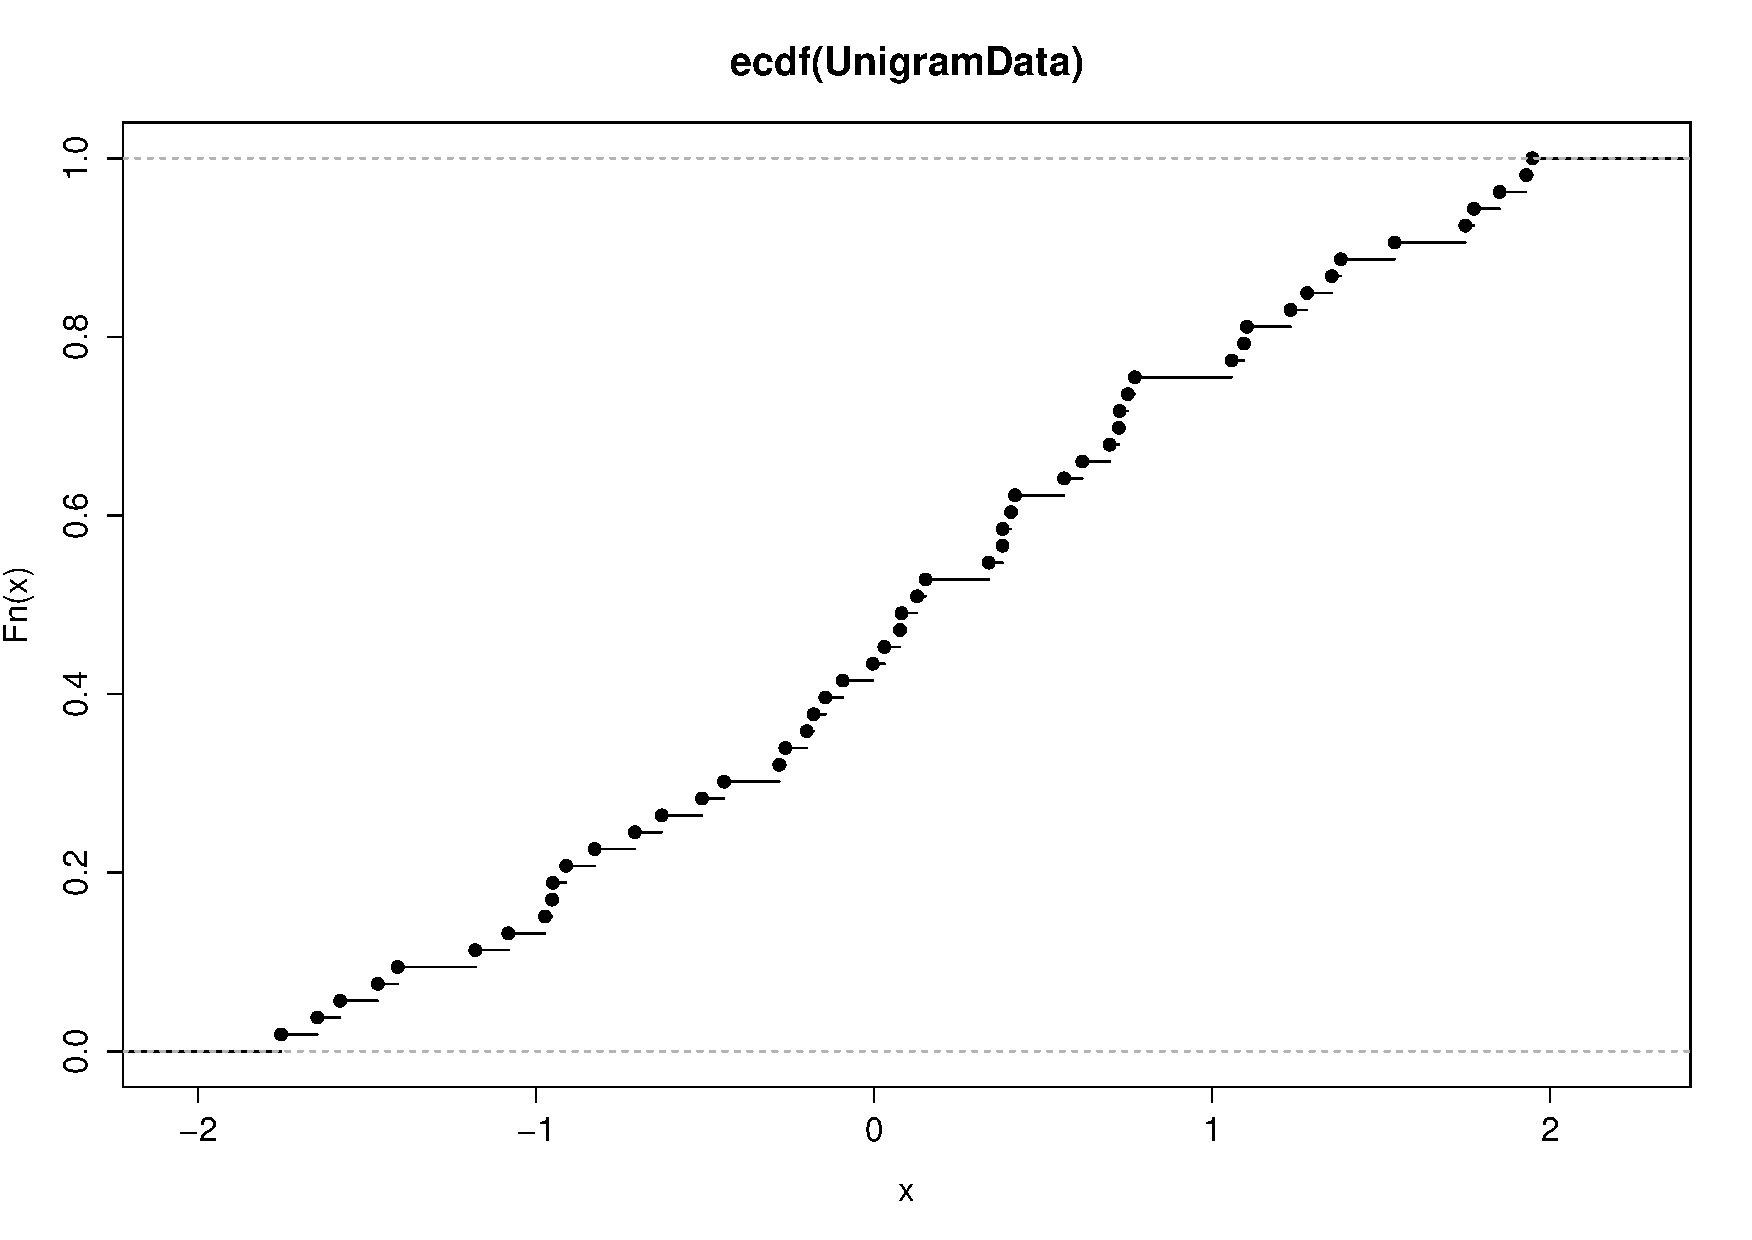
\includegraphics[width=0.8\columnwidth]{unigram} % Example image
\end{center}


\begin{center}
{Figure 2: ECDF OF JACCARD INDEX OF BIGRAMS}
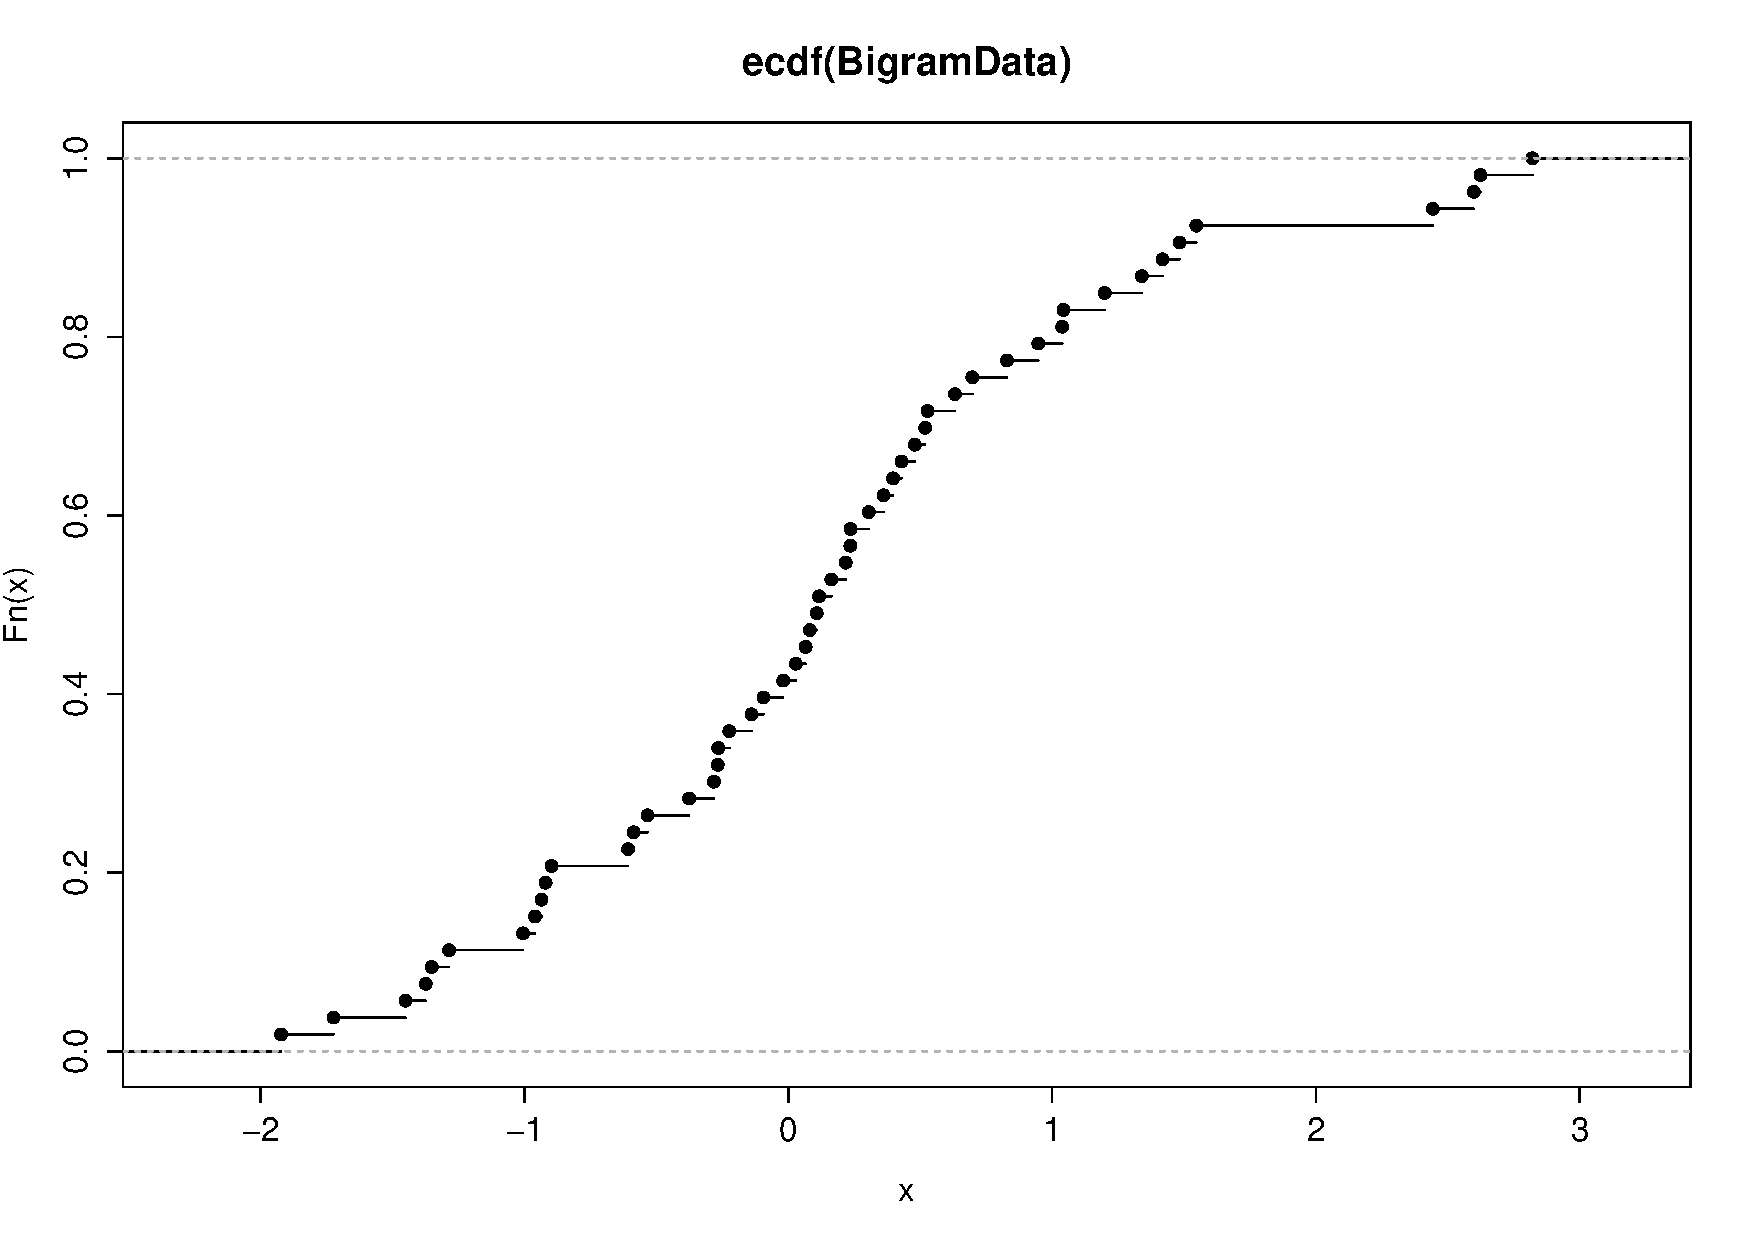
\includegraphics[width=0.8\columnwidth]{bigram} % Example image
\end{center}

\begin{center}
{Figure 3: ECDF OF JACCARD INDEX OF 3-GRAMS}
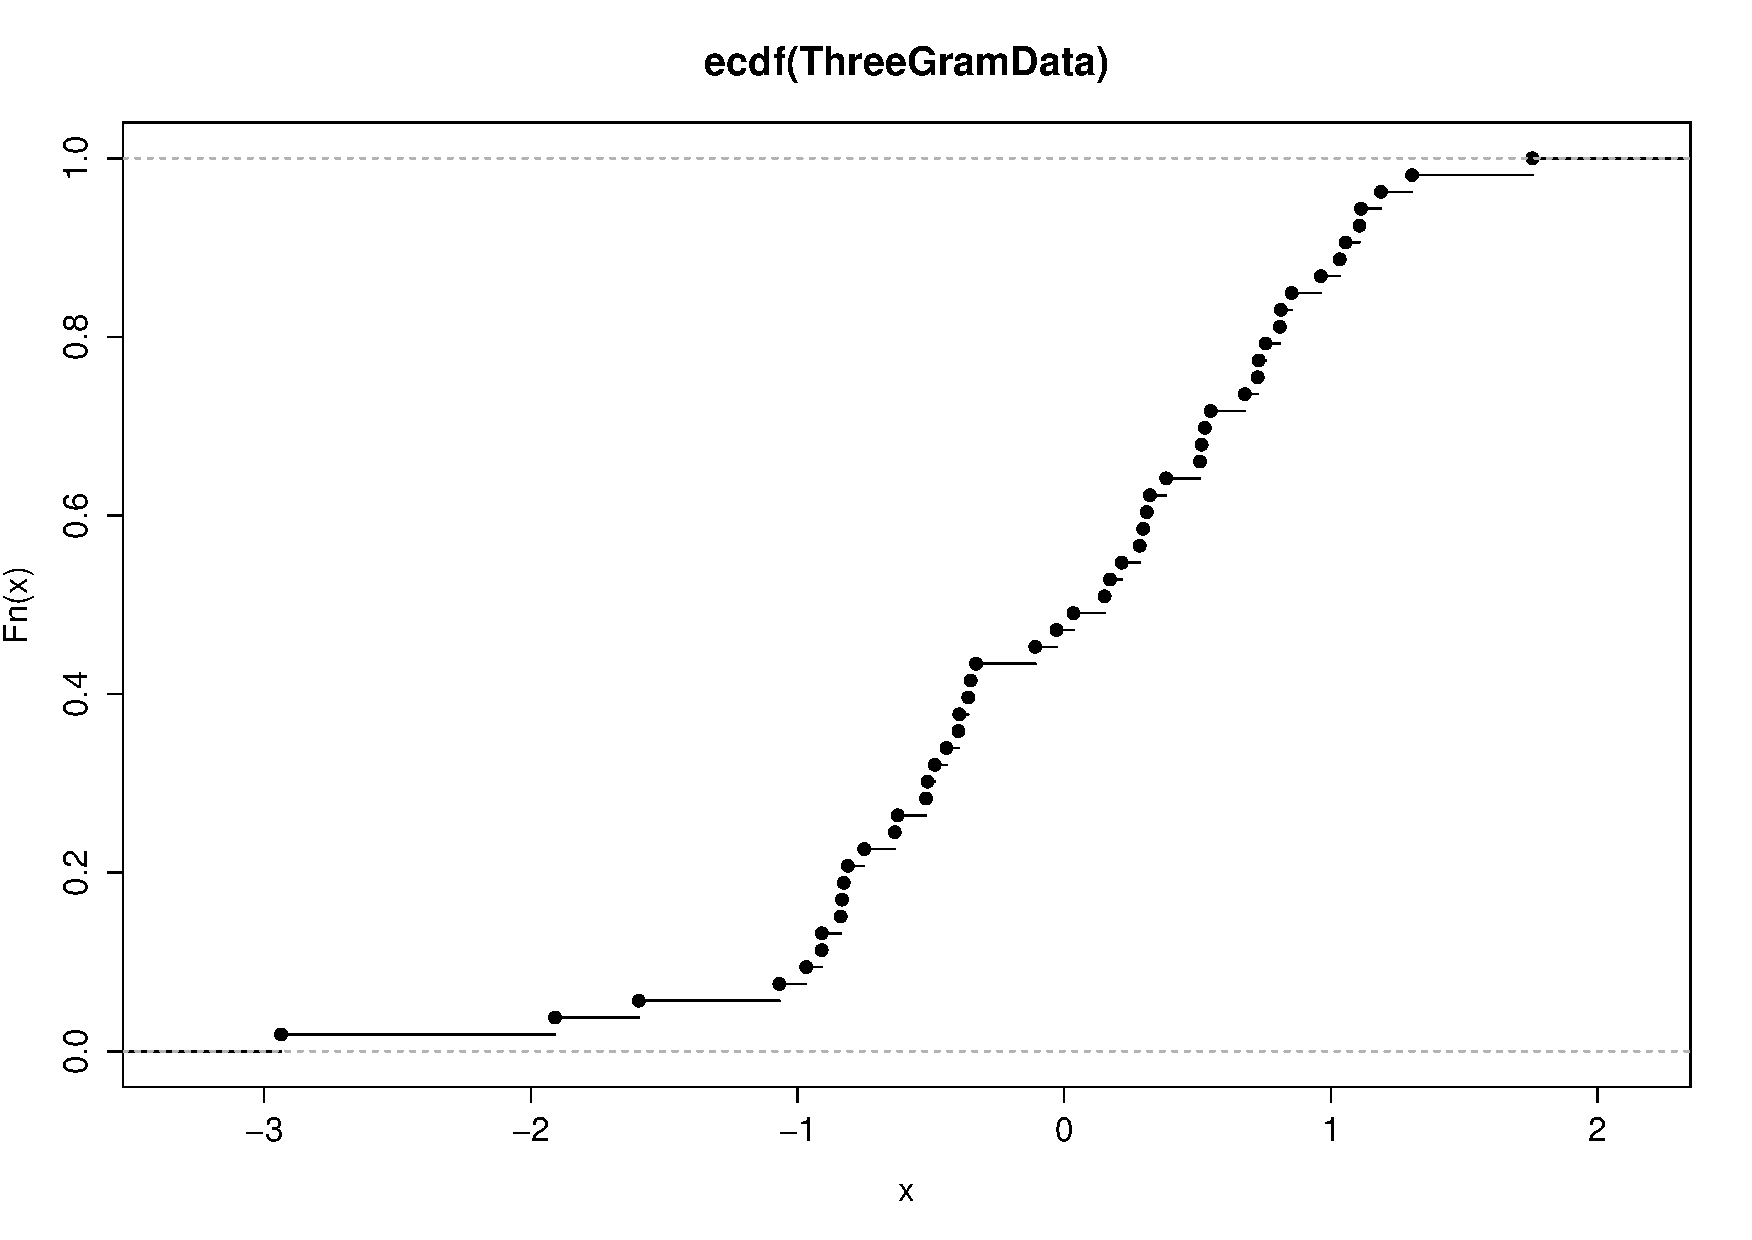
\includegraphics[width=0.8\columnwidth]{3gram} % Example image
\end{center}


\end{homeworkProblem}

%----------------------------------------------------------------------------------------
%	PROBLEM 2
%----------------------------------------------------------------------------------------

\begin{homeworkProblem}

Using the pages from Q1 (A4), download all TimeMaps (including TimeMaps with 404 responses, i.e. empty or null TimeMaps)

\pythonscript{timeMap}{Script To Download TimeMapsPages and Count Mementos(It is used to count all mementos now.)}
\begin{center}
{Figure 4: ECDF OF Total Memento Count}
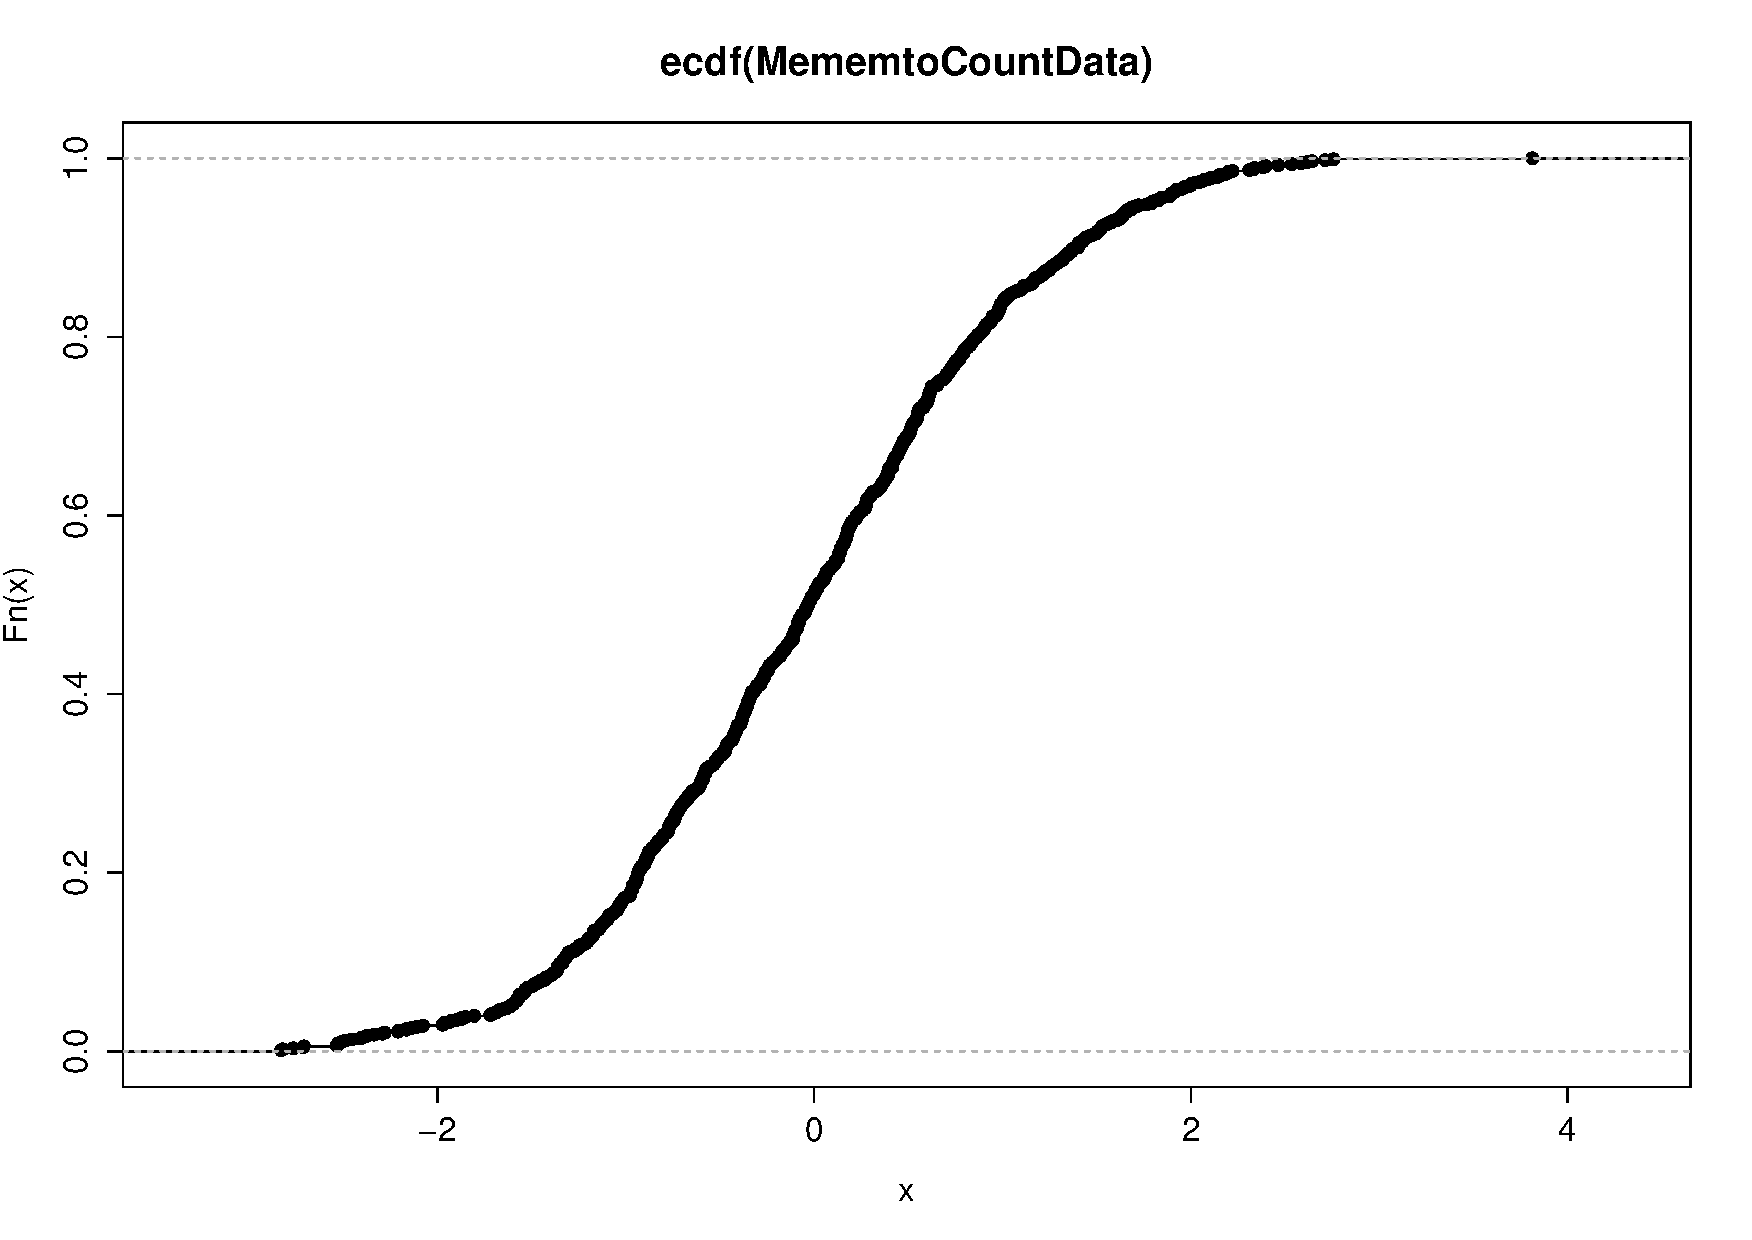
\includegraphics[width=0.8\columnwidth]{mem_count} % Example image
\end{center}



\end{homeworkProblem}

%----------------------------------------------------------------------------------------
%   PROBLEM 3
%----------------------------------------------------------------------------------------
\begin{homeworkProblem}
Using 20 links that have TimeMaps
With greater than or = 20 mementos
Have existed greater than or = 2 years (i.e., Memento-Datetime of “first memento” is April XX, 2013 or older)
Note: select from Q1/Q2 links, else choose them by hand
For each link, create a graph that shows Jaccard Distance, relative to the first memento, through time
x-axis: continuous time, y-axis: Jaccard Distance relative to the first memento

\pythonscript{memento_jack}{Script For Q3}

\begin{center}
{Figure 5: JACCARD INDEX Assuming Contant Time for First URI}
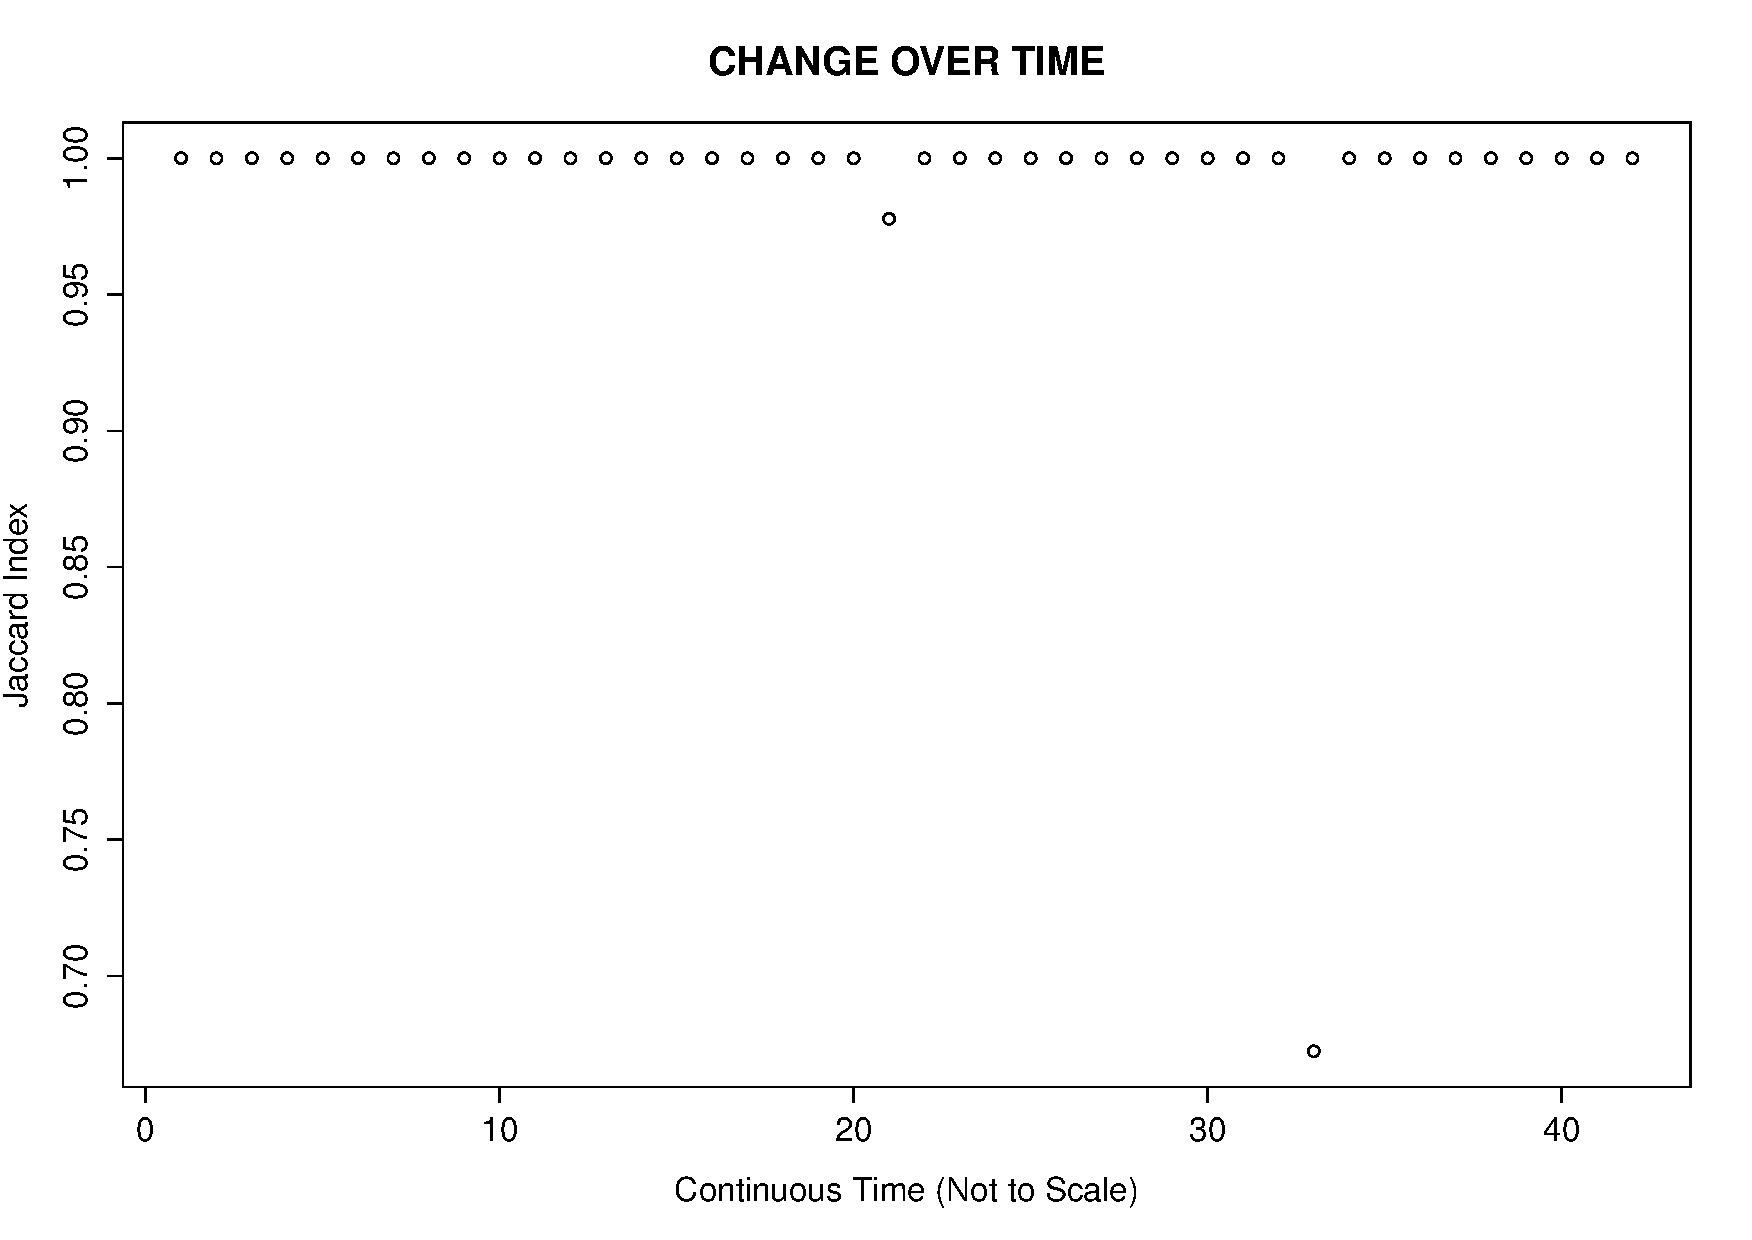
\includegraphics[width=0.8\columnwidth]{first} % Example image
\end{center}

\begin{center}
{Figure 6: JACCARD INDEX Assuming Contant Time for Second URI}
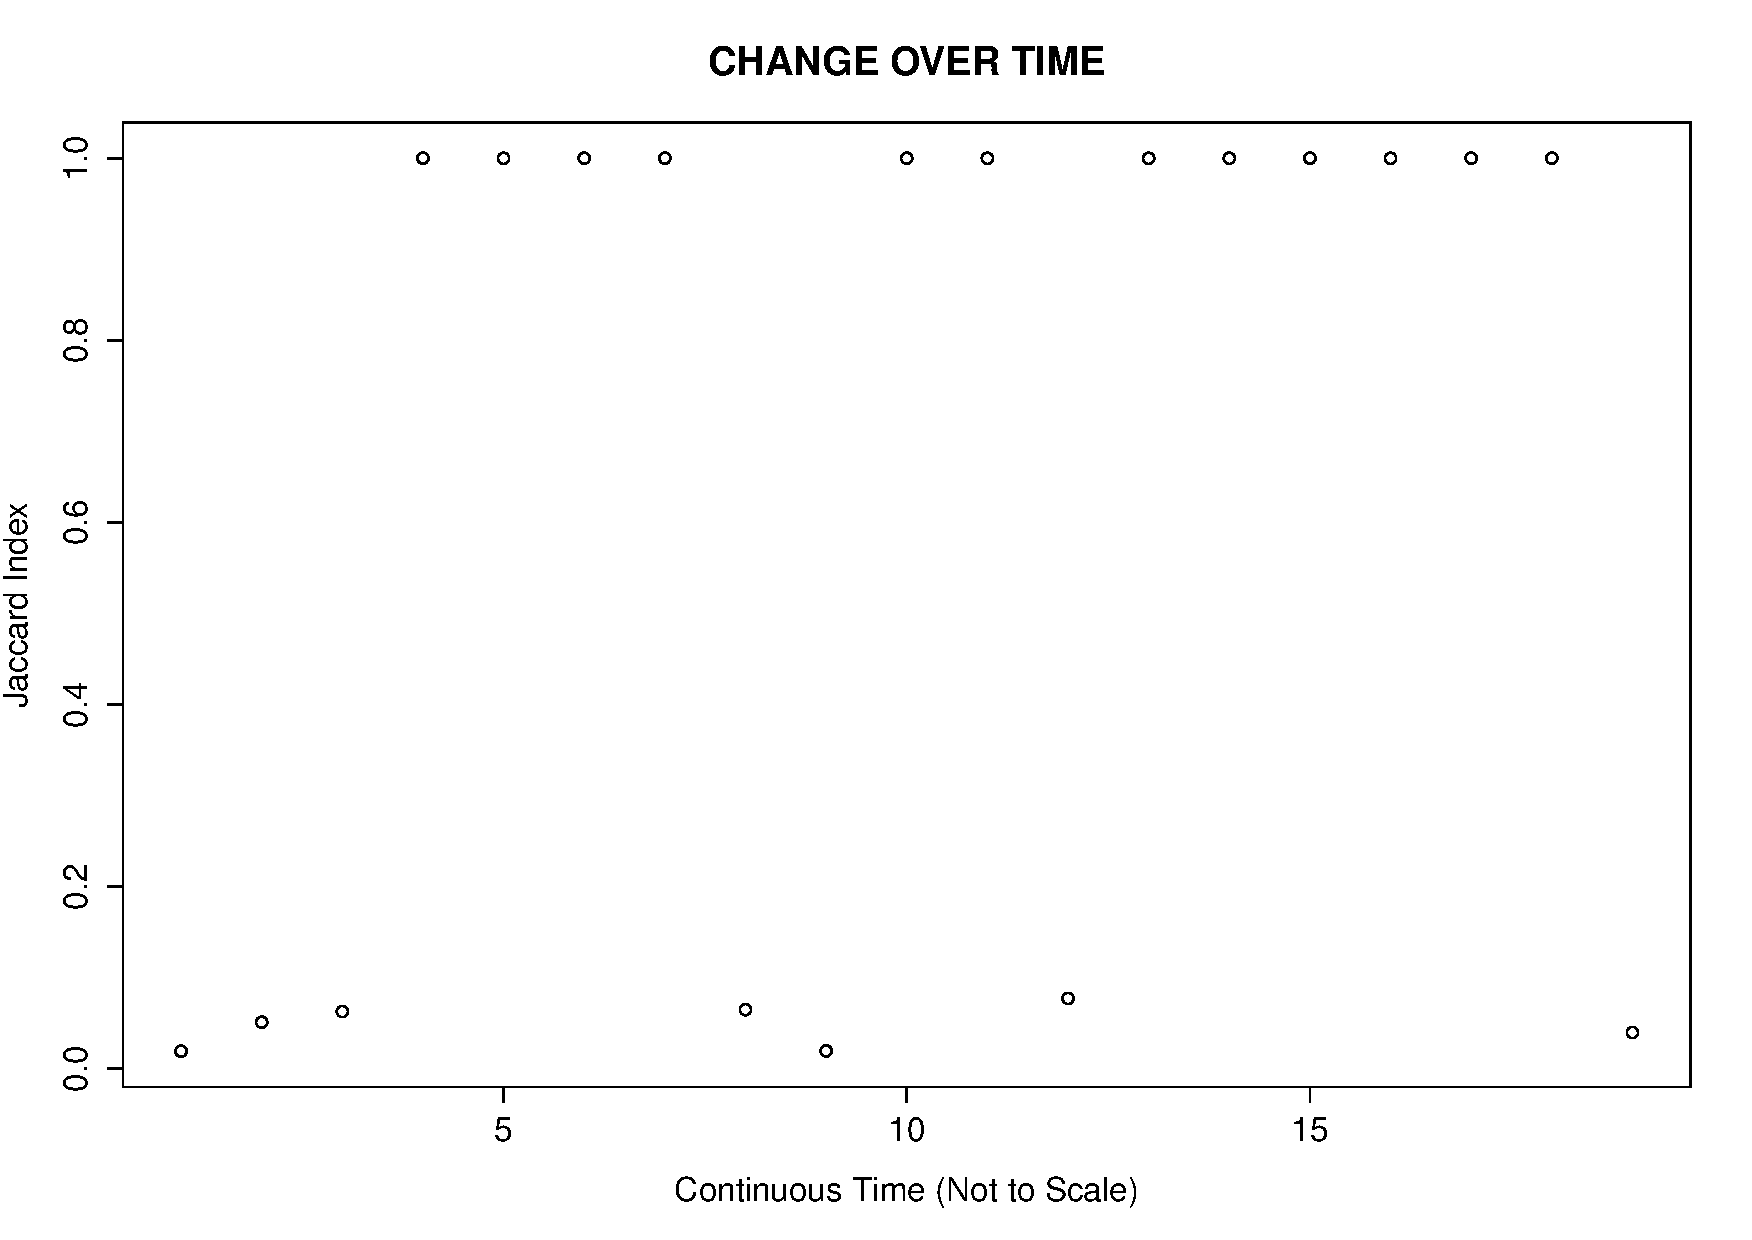
\includegraphics[width=0.8\columnwidth]{second} % Example image
\end{center}

\begin{center}
{Figure 7: JACCARD INDEX Assuming Contant Time for Third URI}
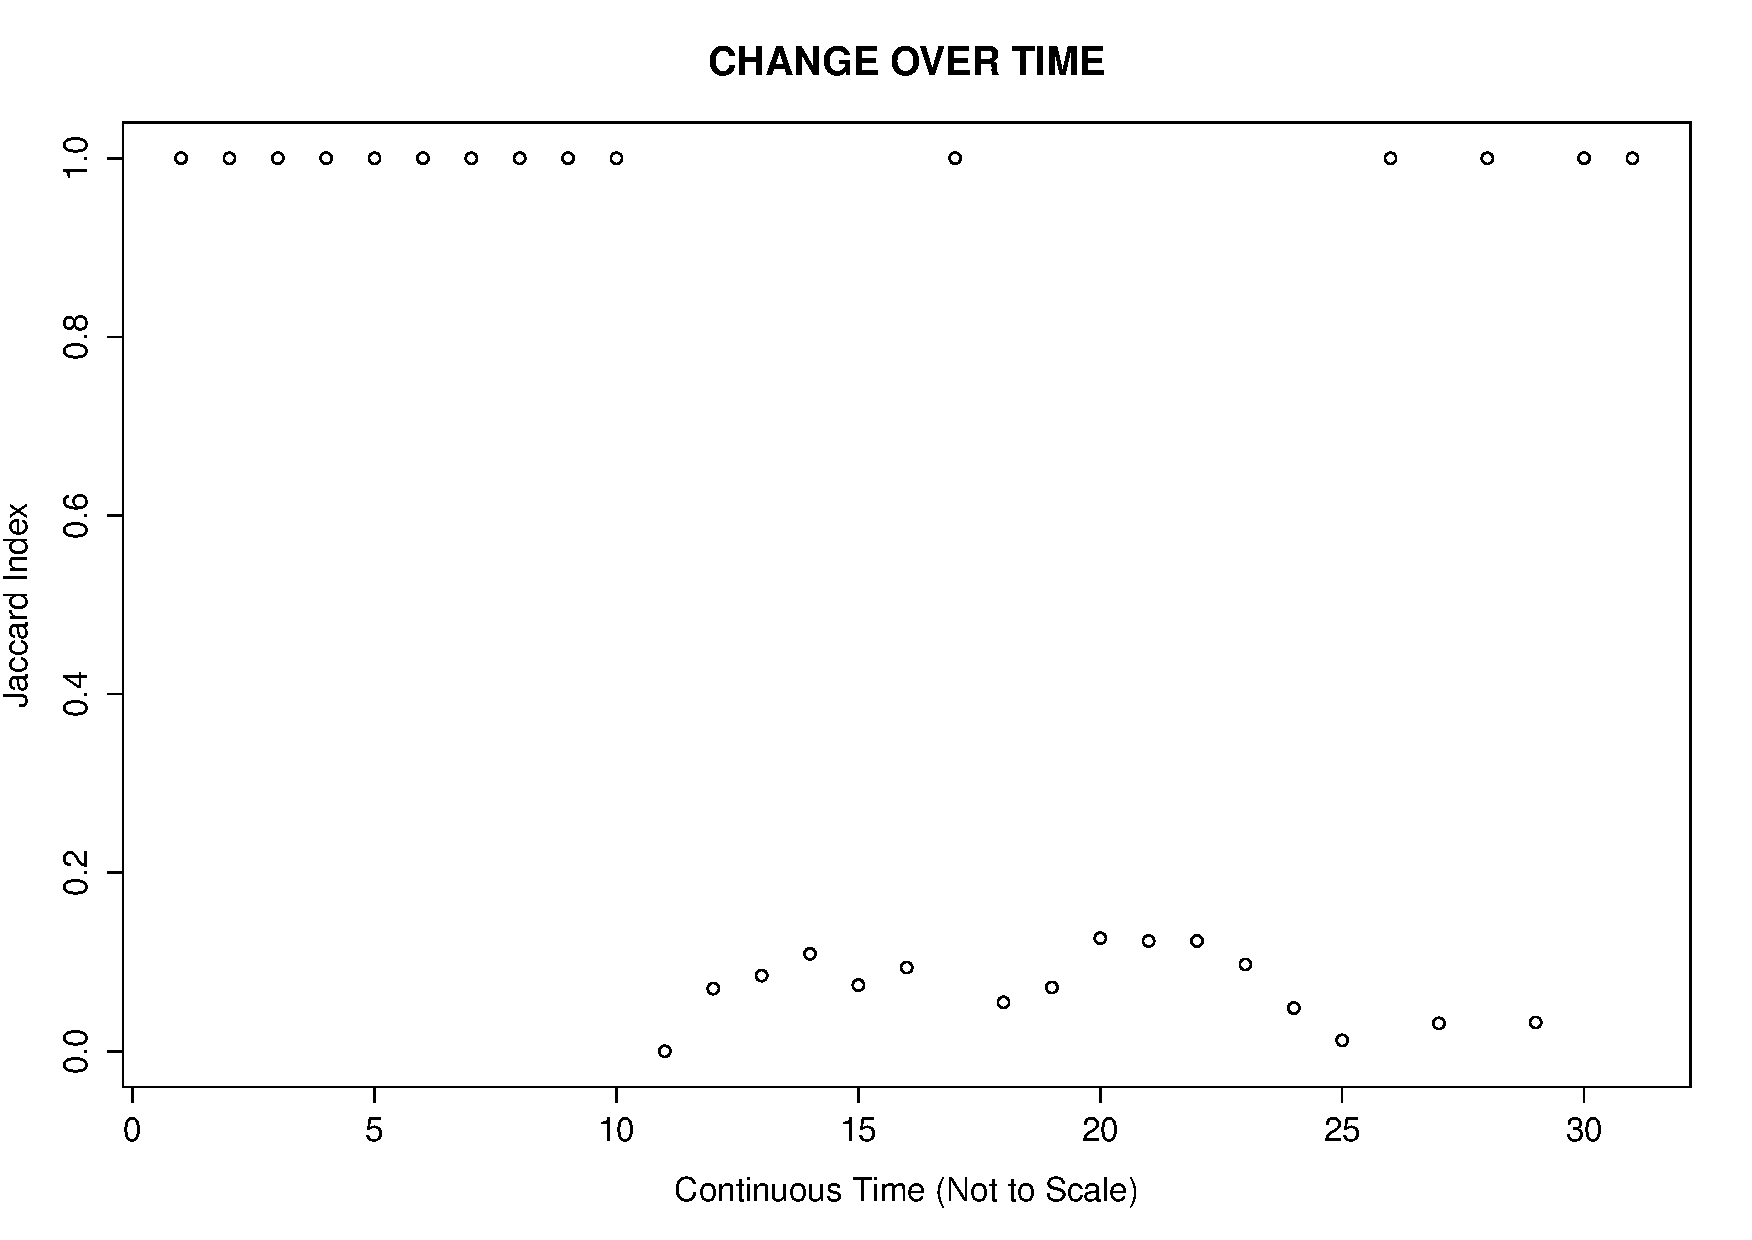
\includegraphics[width=0.8\columnwidth]{third} % Example image
\end{center}

\begin{center}
{Figure 8: JACCARD INDEX Assuming Contant Time for Fourth URI}
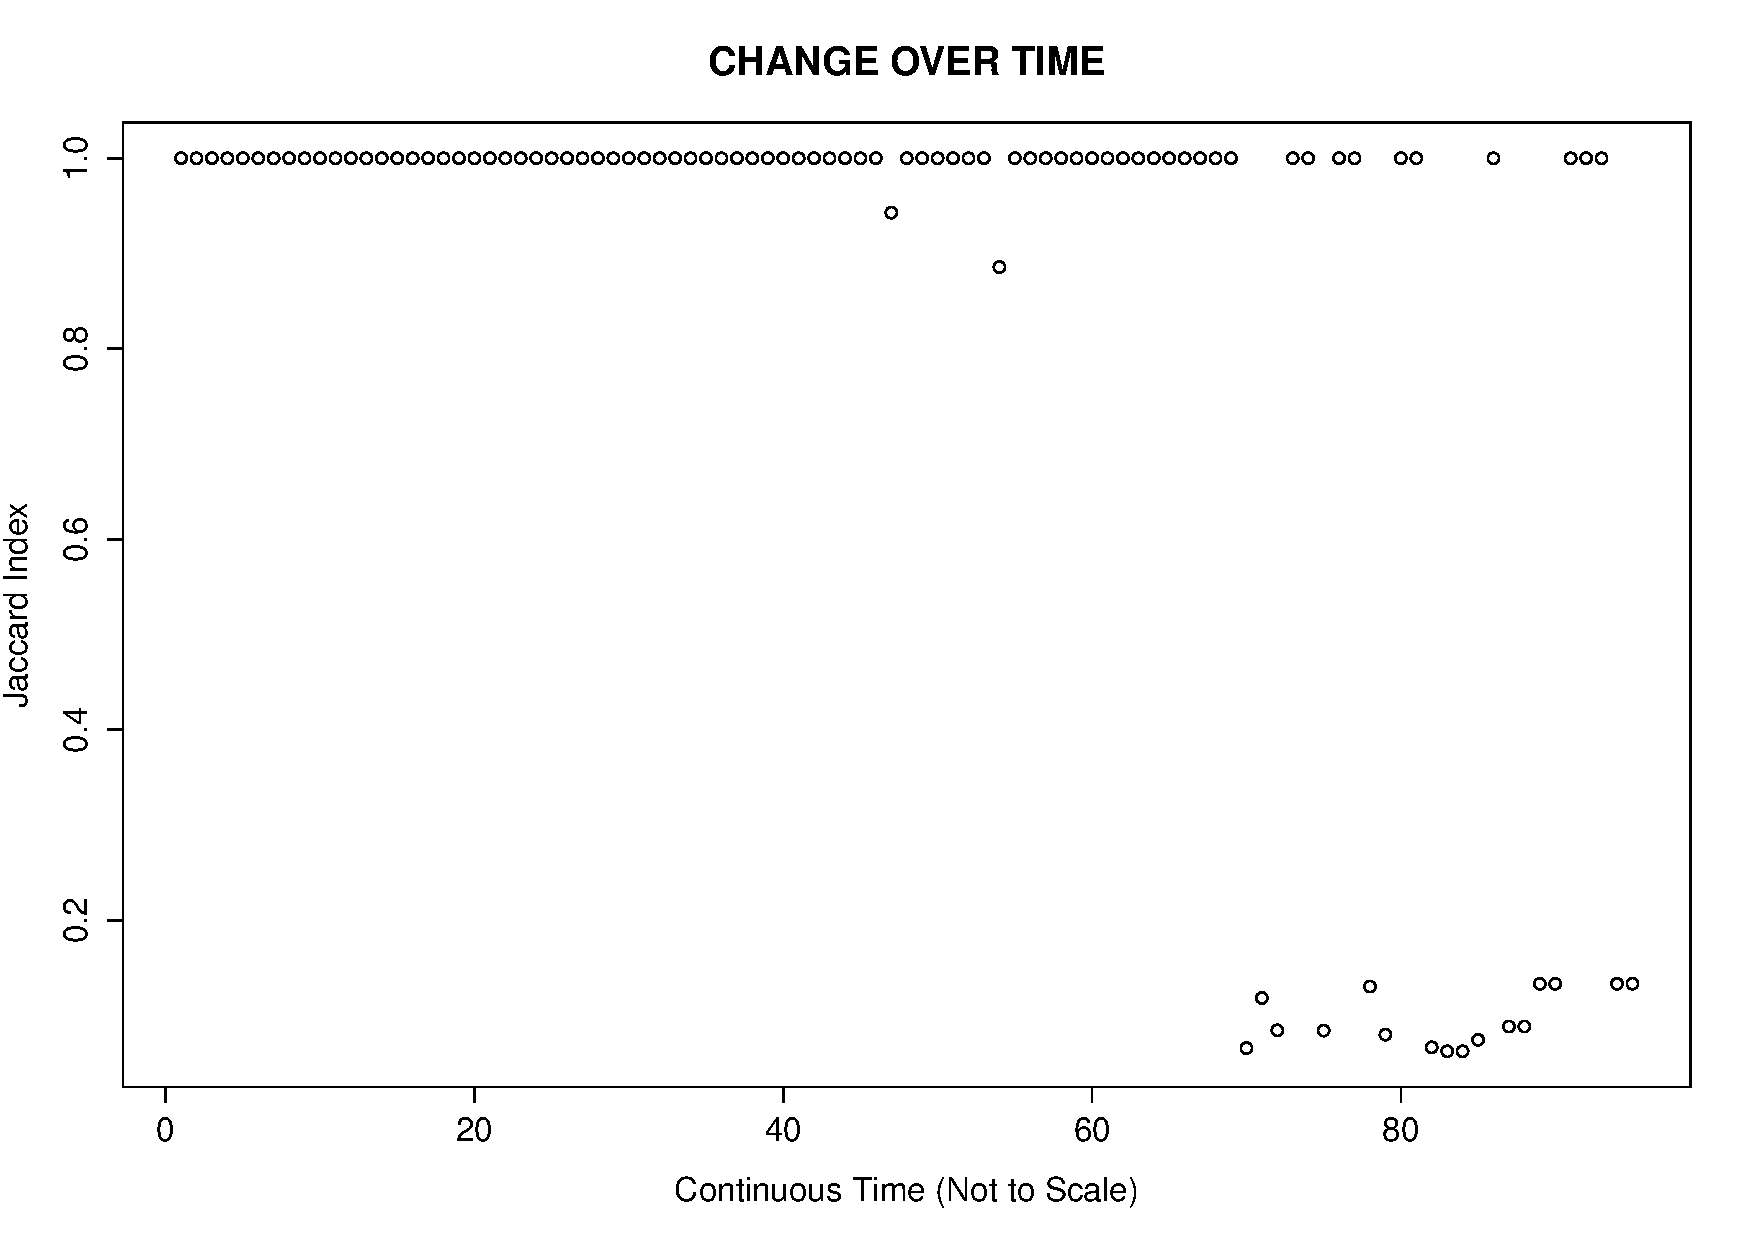
\includegraphics[width=0.8\columnwidth]{fourth} % Example image
\end{center}

\begin{center}
{Figure 9: JACCARD INDEX Assuming Contant Time for Fifth URI}
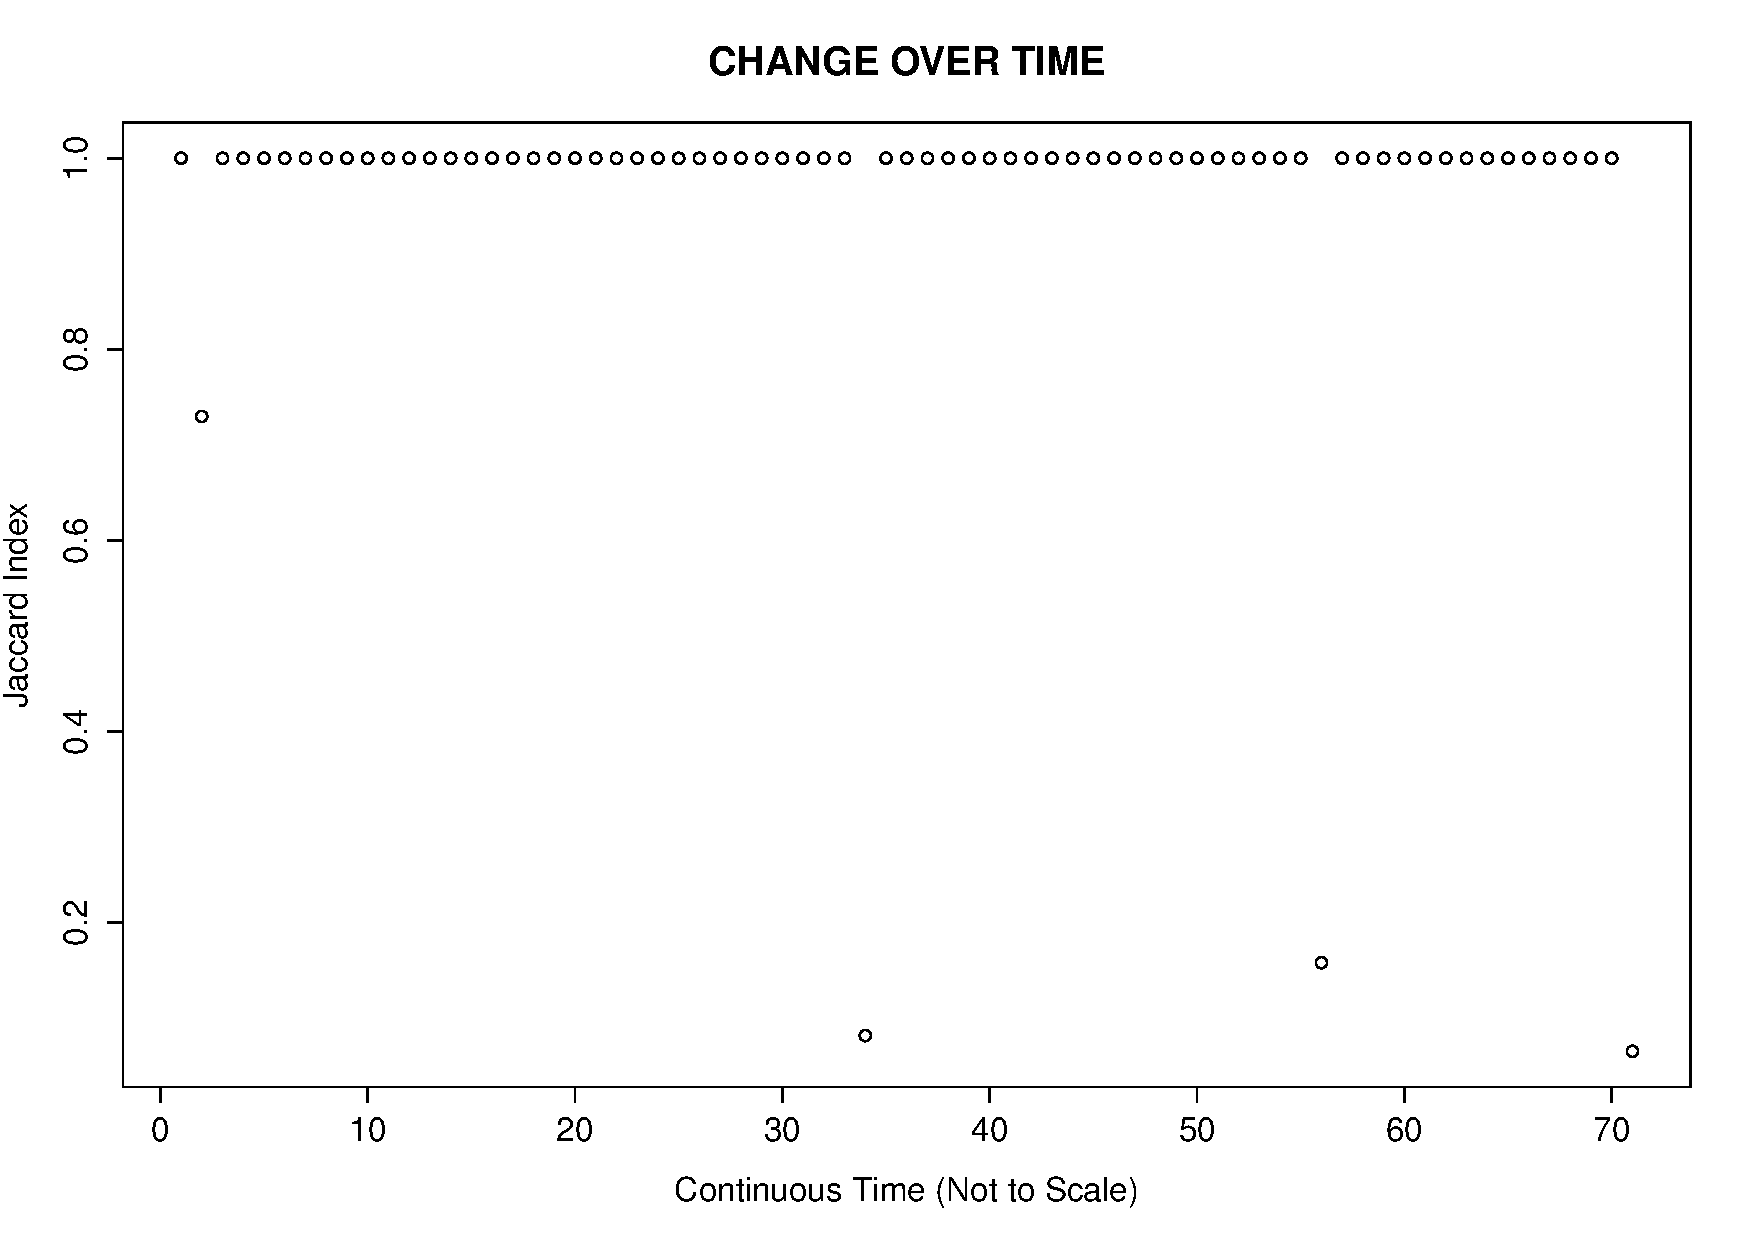
\includegraphics[width=0.8\columnwidth]{fifth} % Example image
\end{center}

\begin{center}
{Figure 10: JACCARD INDEX Assuming Contant Time for Sixth URI}
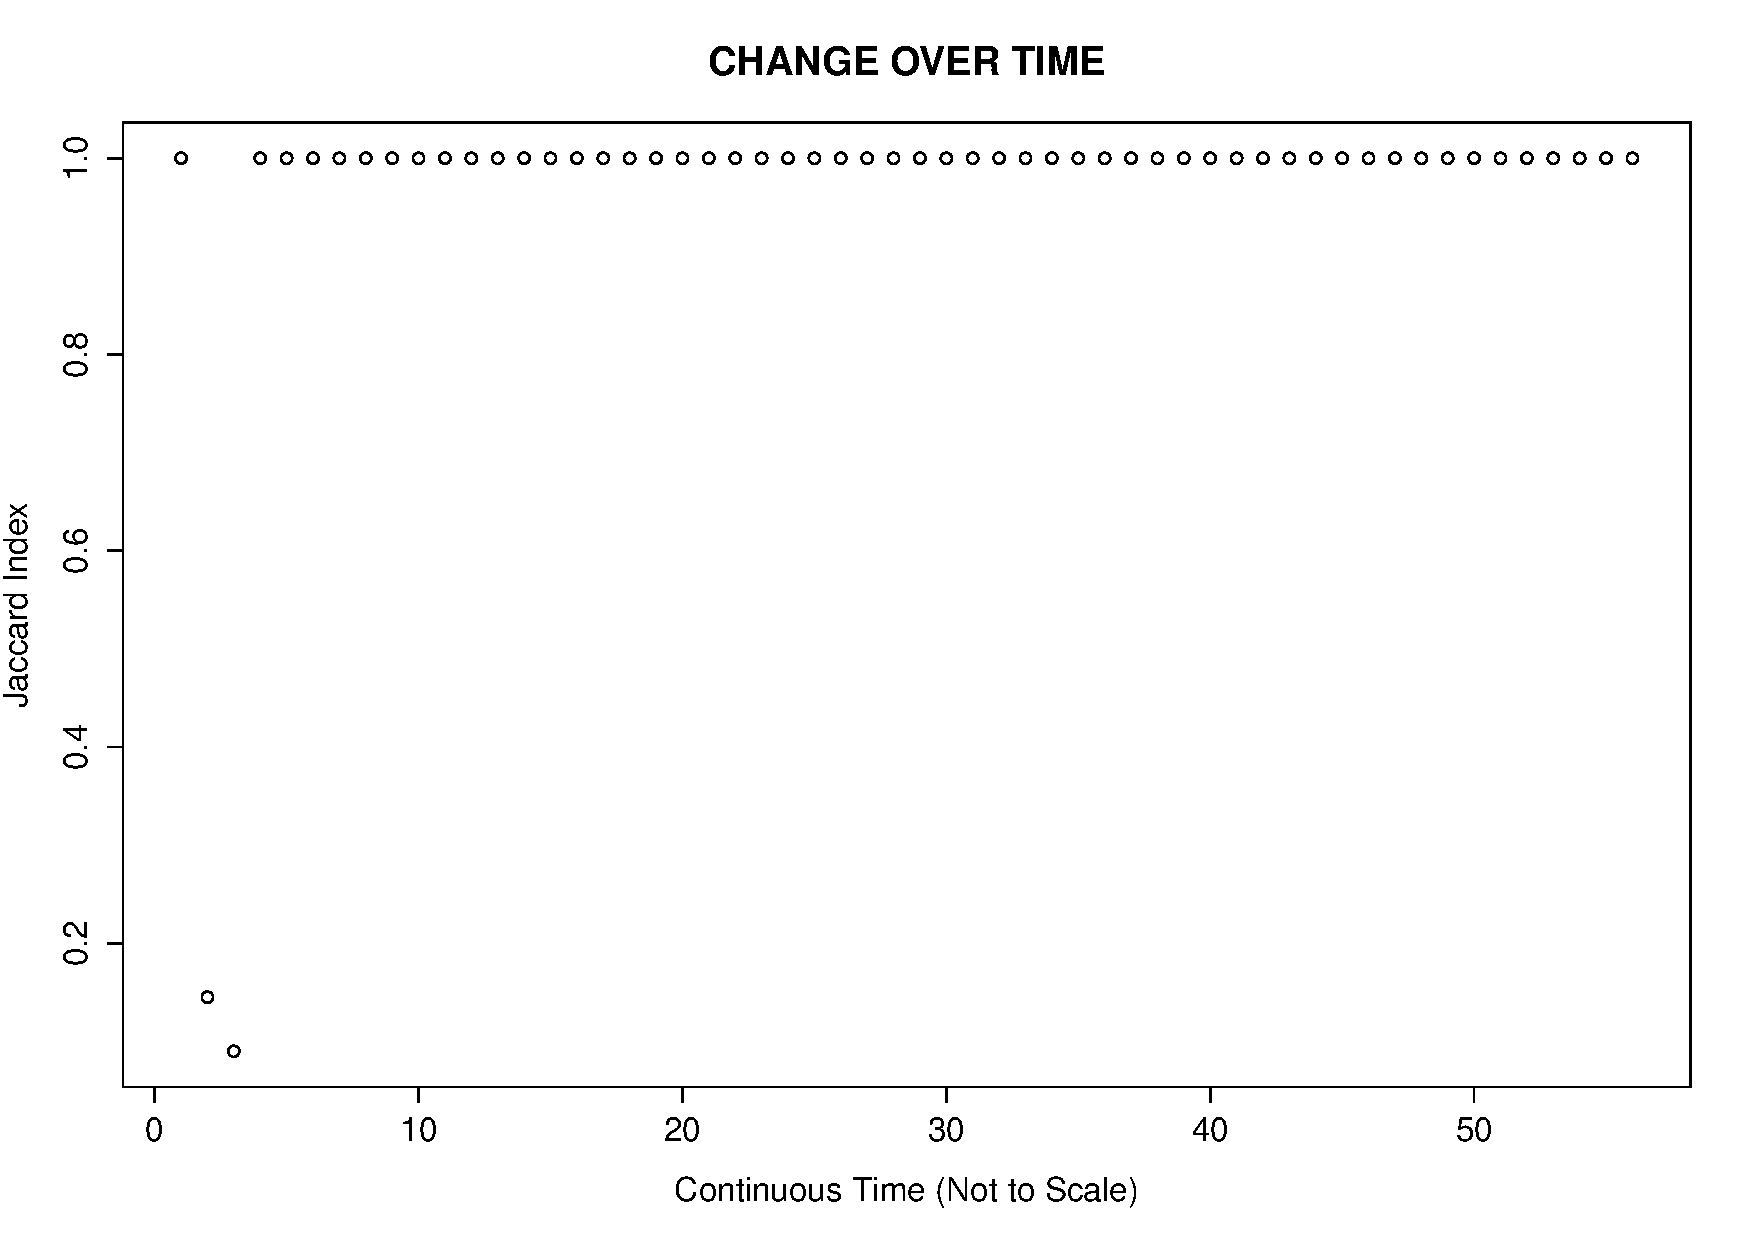
\includegraphics[width=0.8\columnwidth]{Sixth} % Example image
\end{center}

\begin{center}
{Figure 11: JACCARD INDEX Assuming Contant Time for Seventh URI}
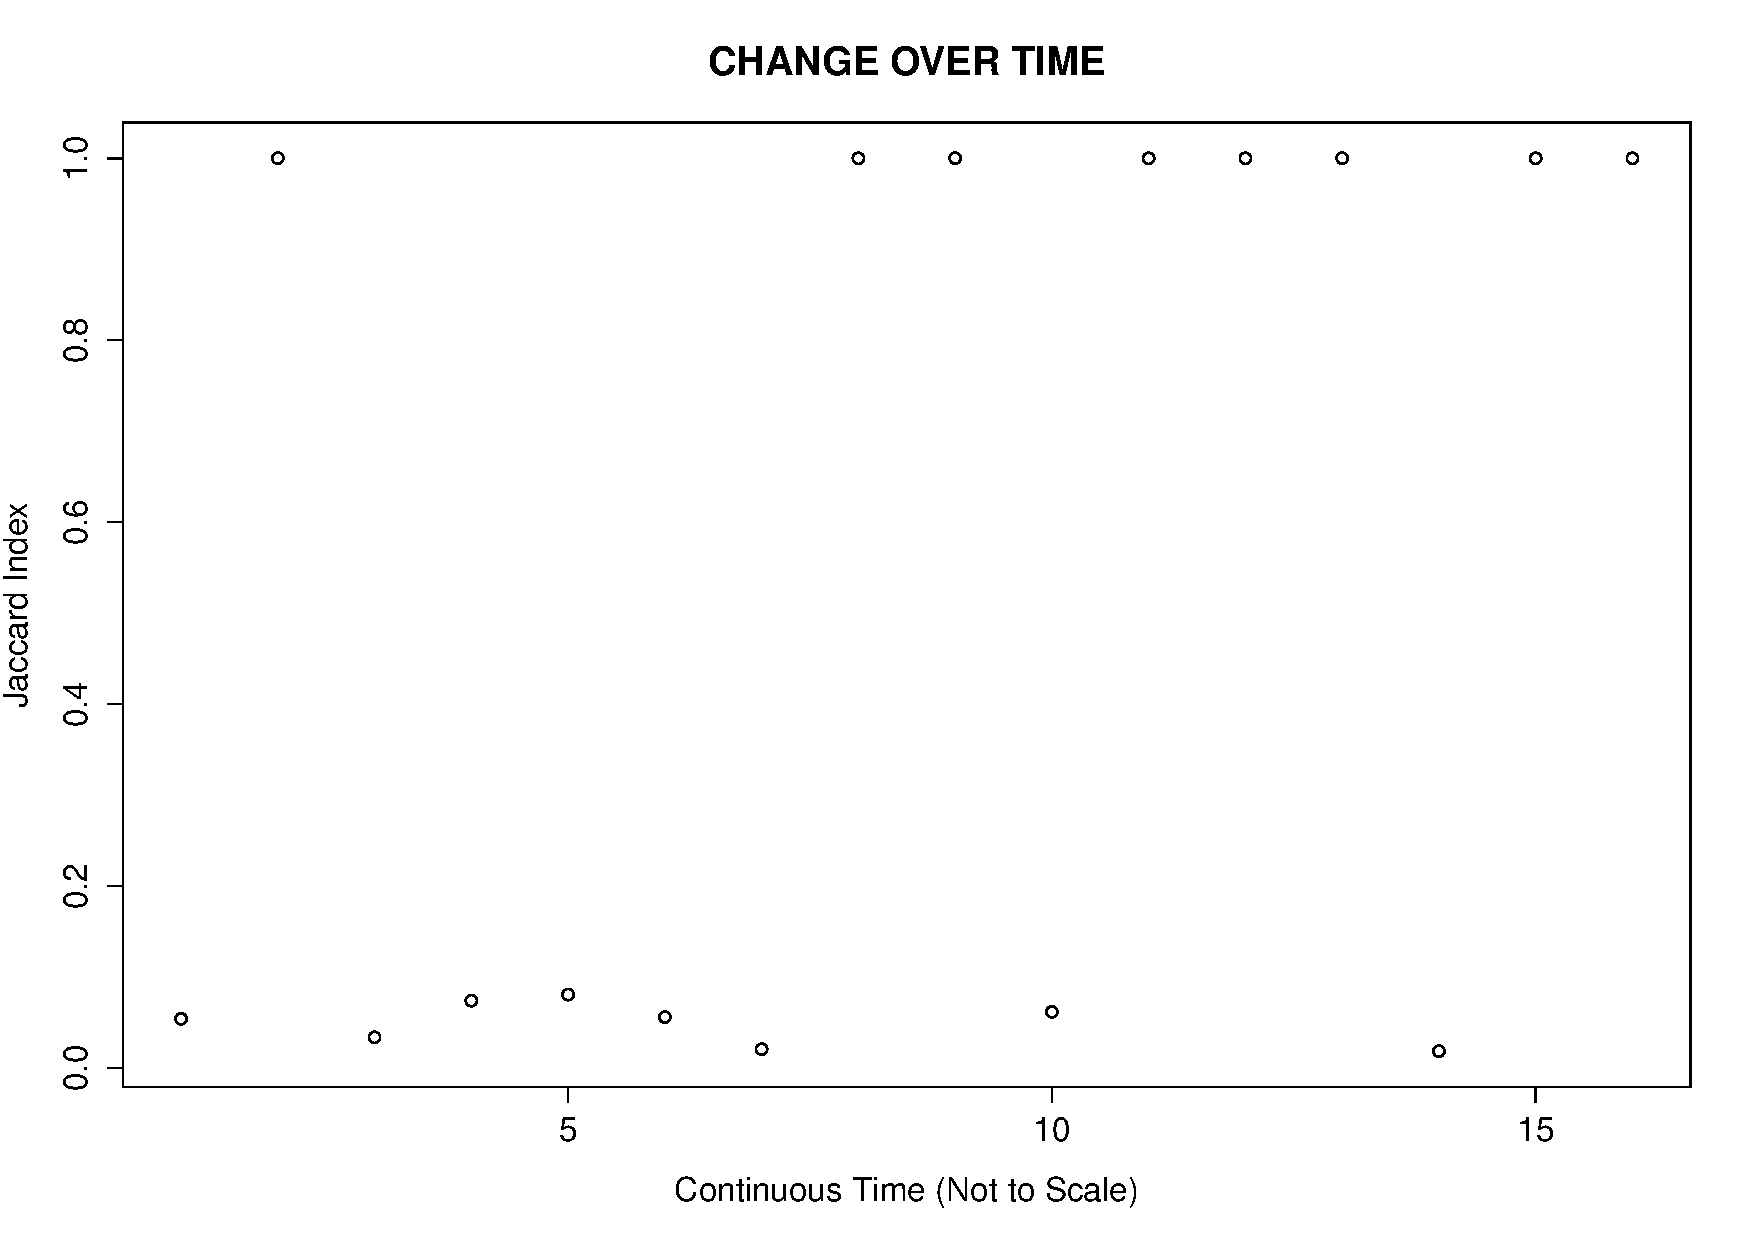
\includegraphics[width=0.8\columnwidth]{Seventh} % Example image
\end{center}

\begin{center}
{Figure 12: JACCARD INDEX Assuming Contant Time for Eight URI}
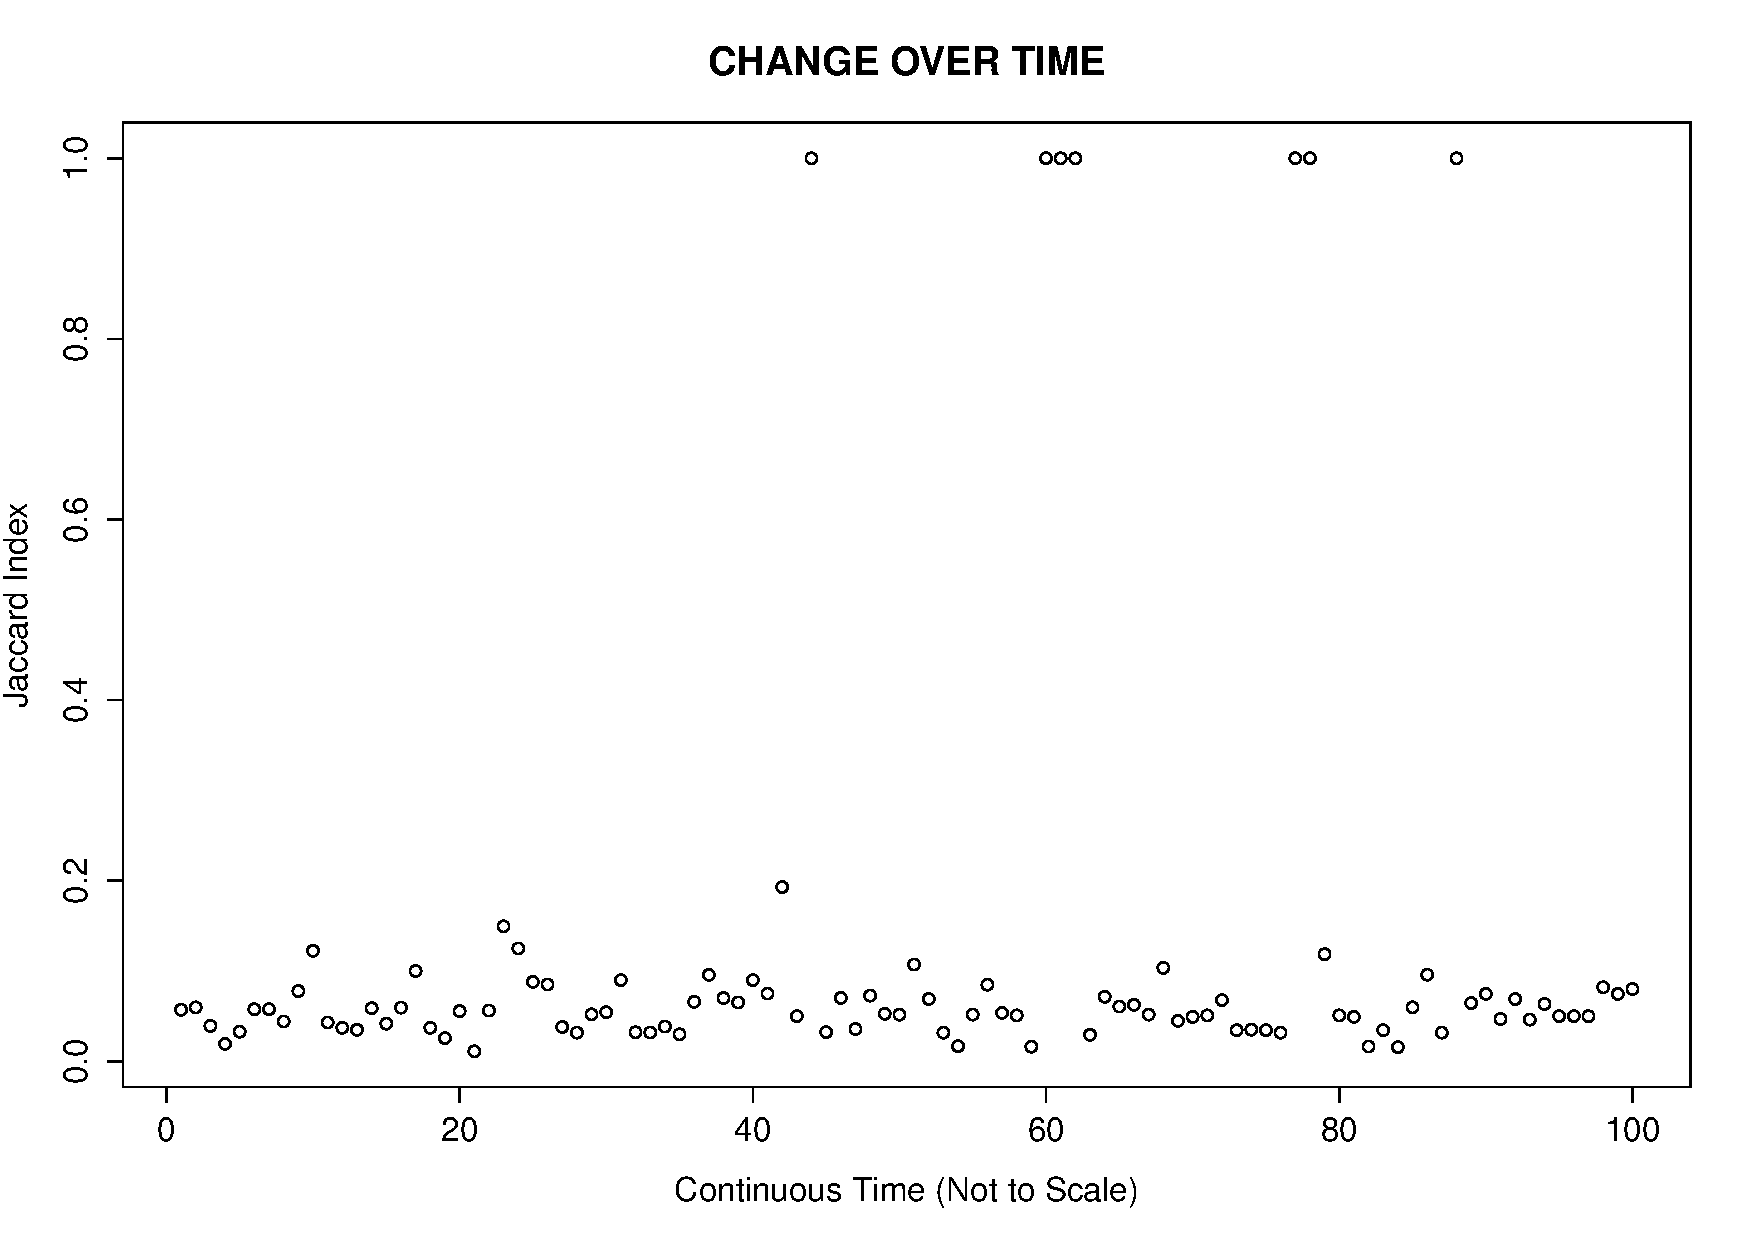
\includegraphics[width=0.8\columnwidth]{eight} % Example image
\end{center}

\begin{center}
{Figure 13: JACCARD INDEX Assuming Contant Time for Ninth URI}
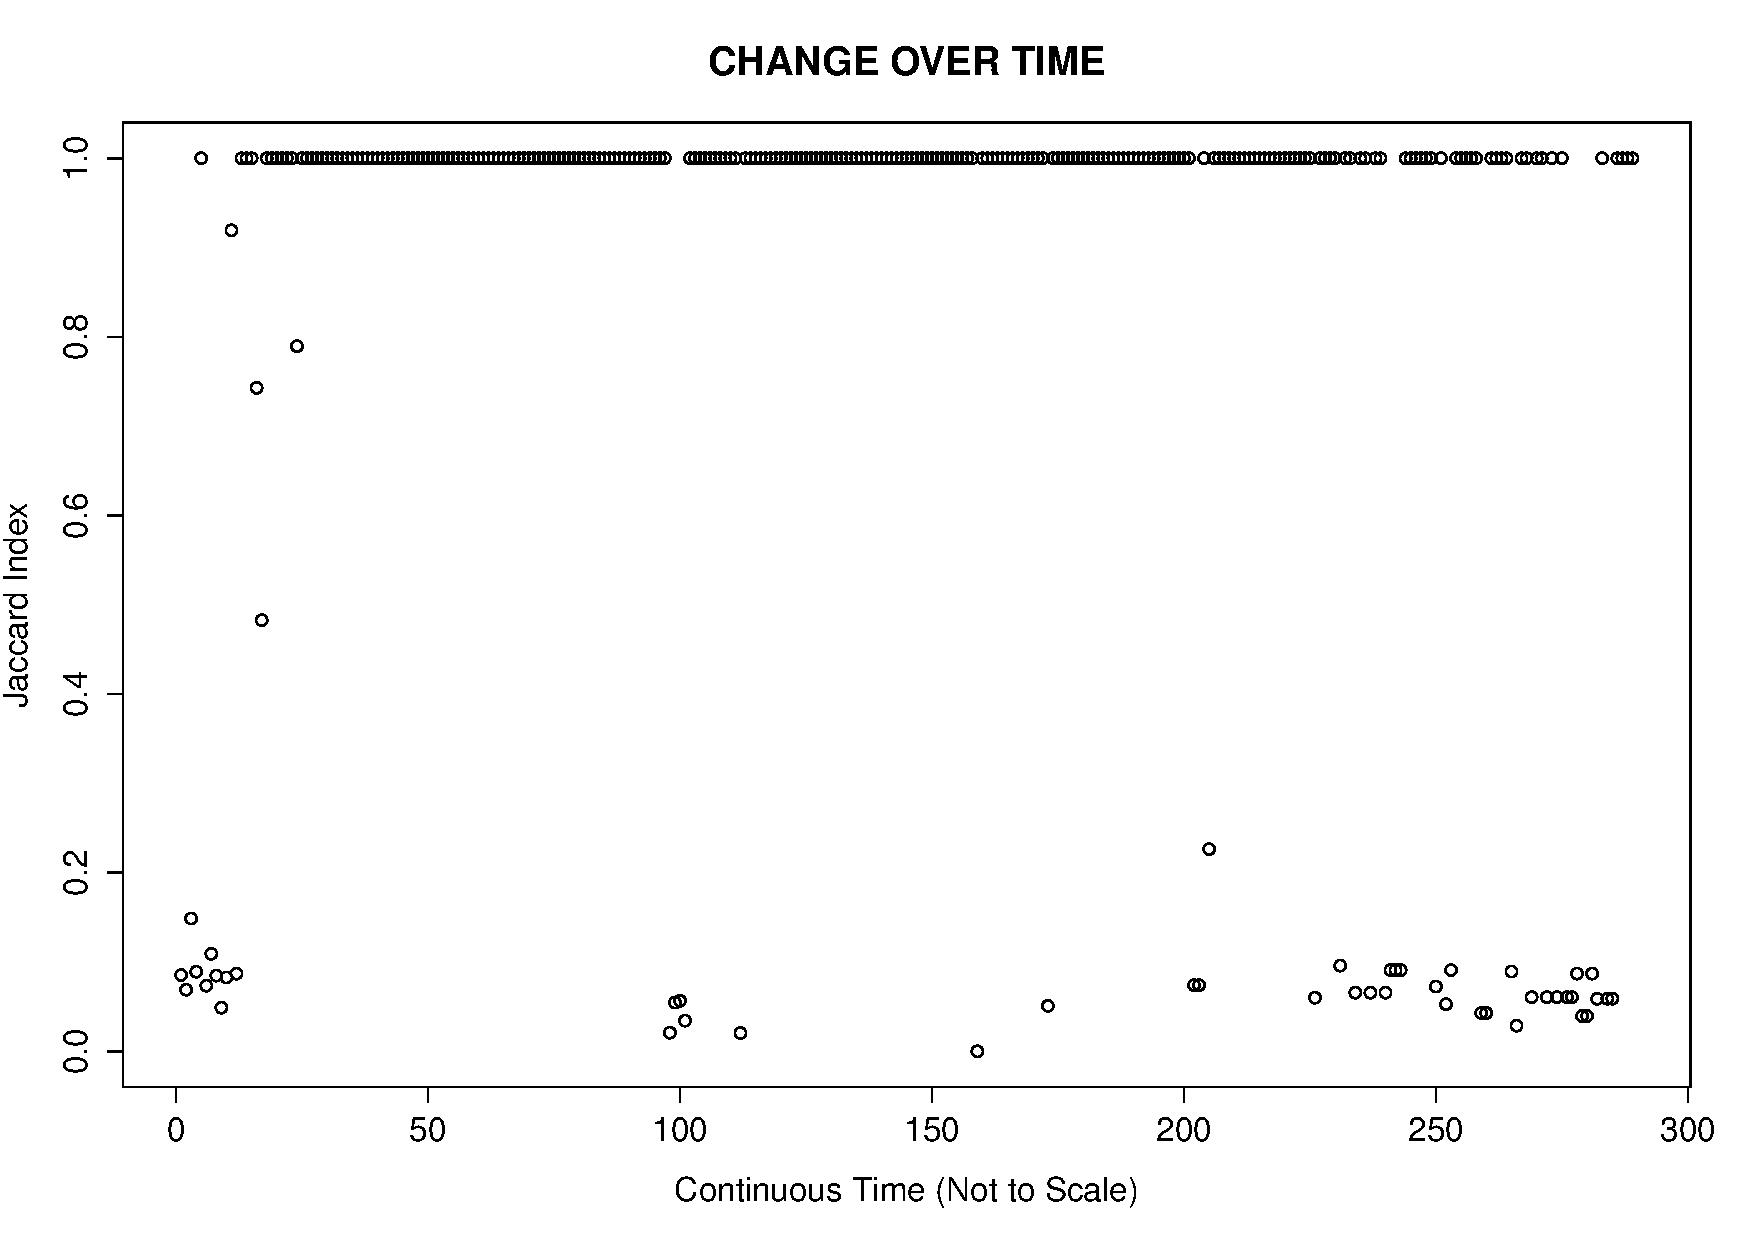
\includegraphics[width=0.8\columnwidth]{ninth} % Example image
\end{center}

\begin{center}
{Figure 14: JACCARD INDEX Assuming Contant Time for Tenth URI}
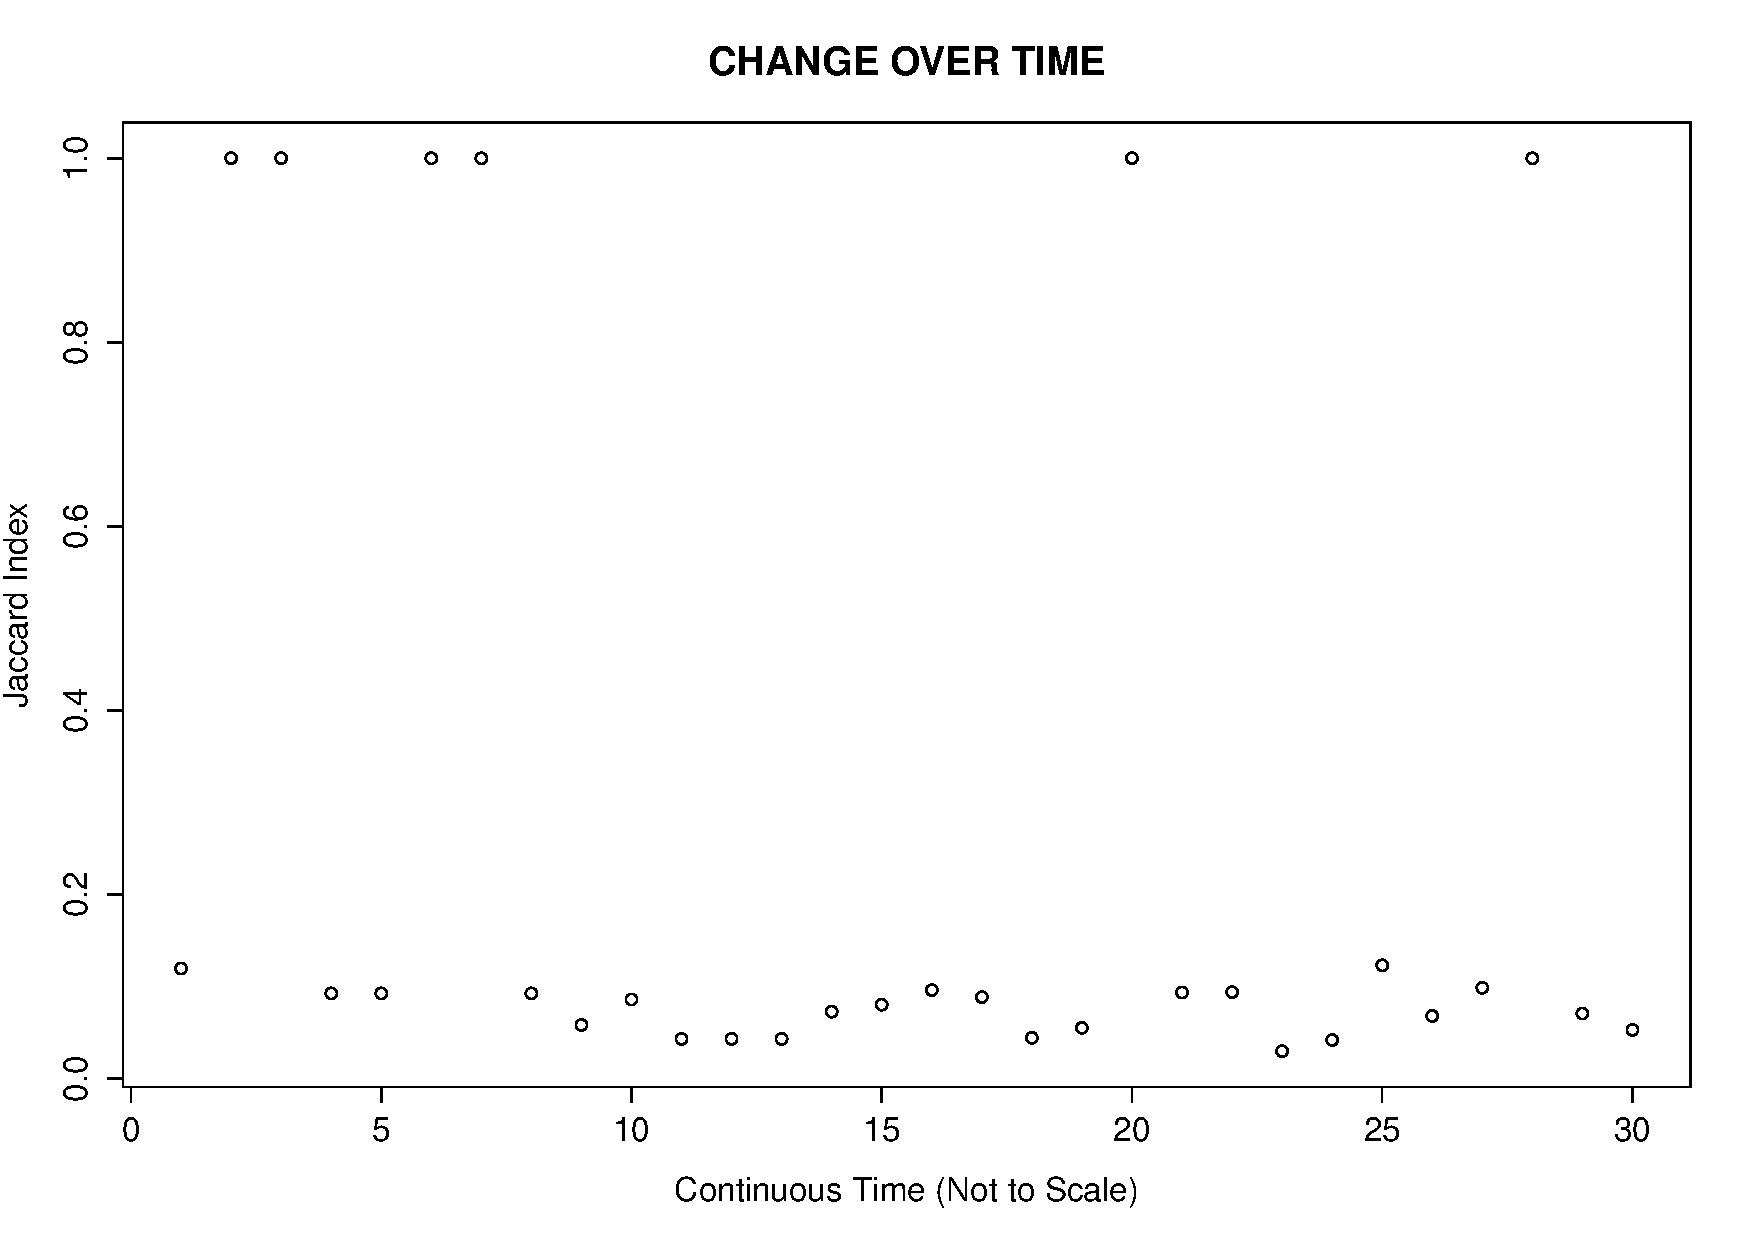
\includegraphics[width=0.8\columnwidth]{tenth} % Example image
\end{center}

\begin{center}
{Figure 15: JACCARD INDEX Assuming Contant Time for Eleventh URI}
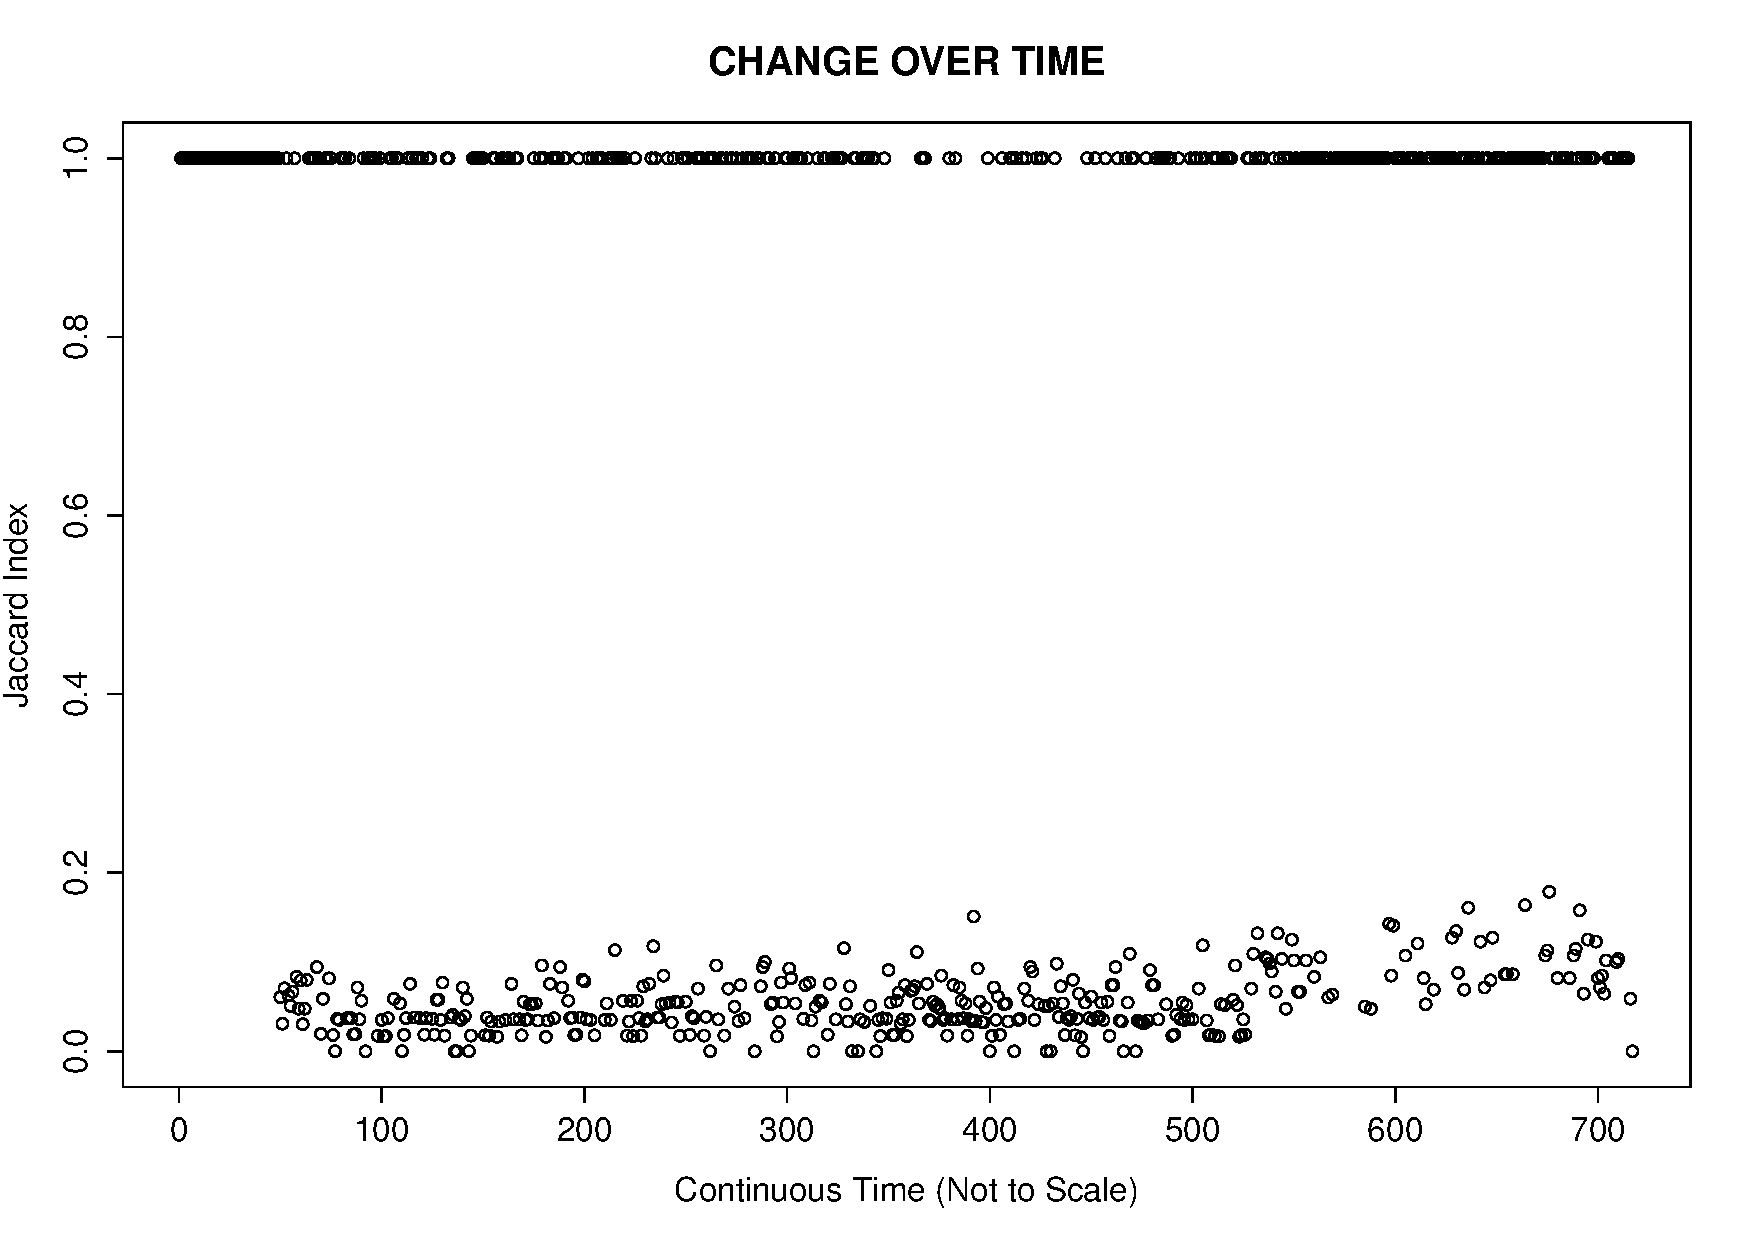
\includegraphics[width=0.8\columnwidth]{eleventh} % Example image
\end{center}

\begin{center}
{Figure 16: JACCARD INDEX Assuming Contant Time for Twelveth URI}
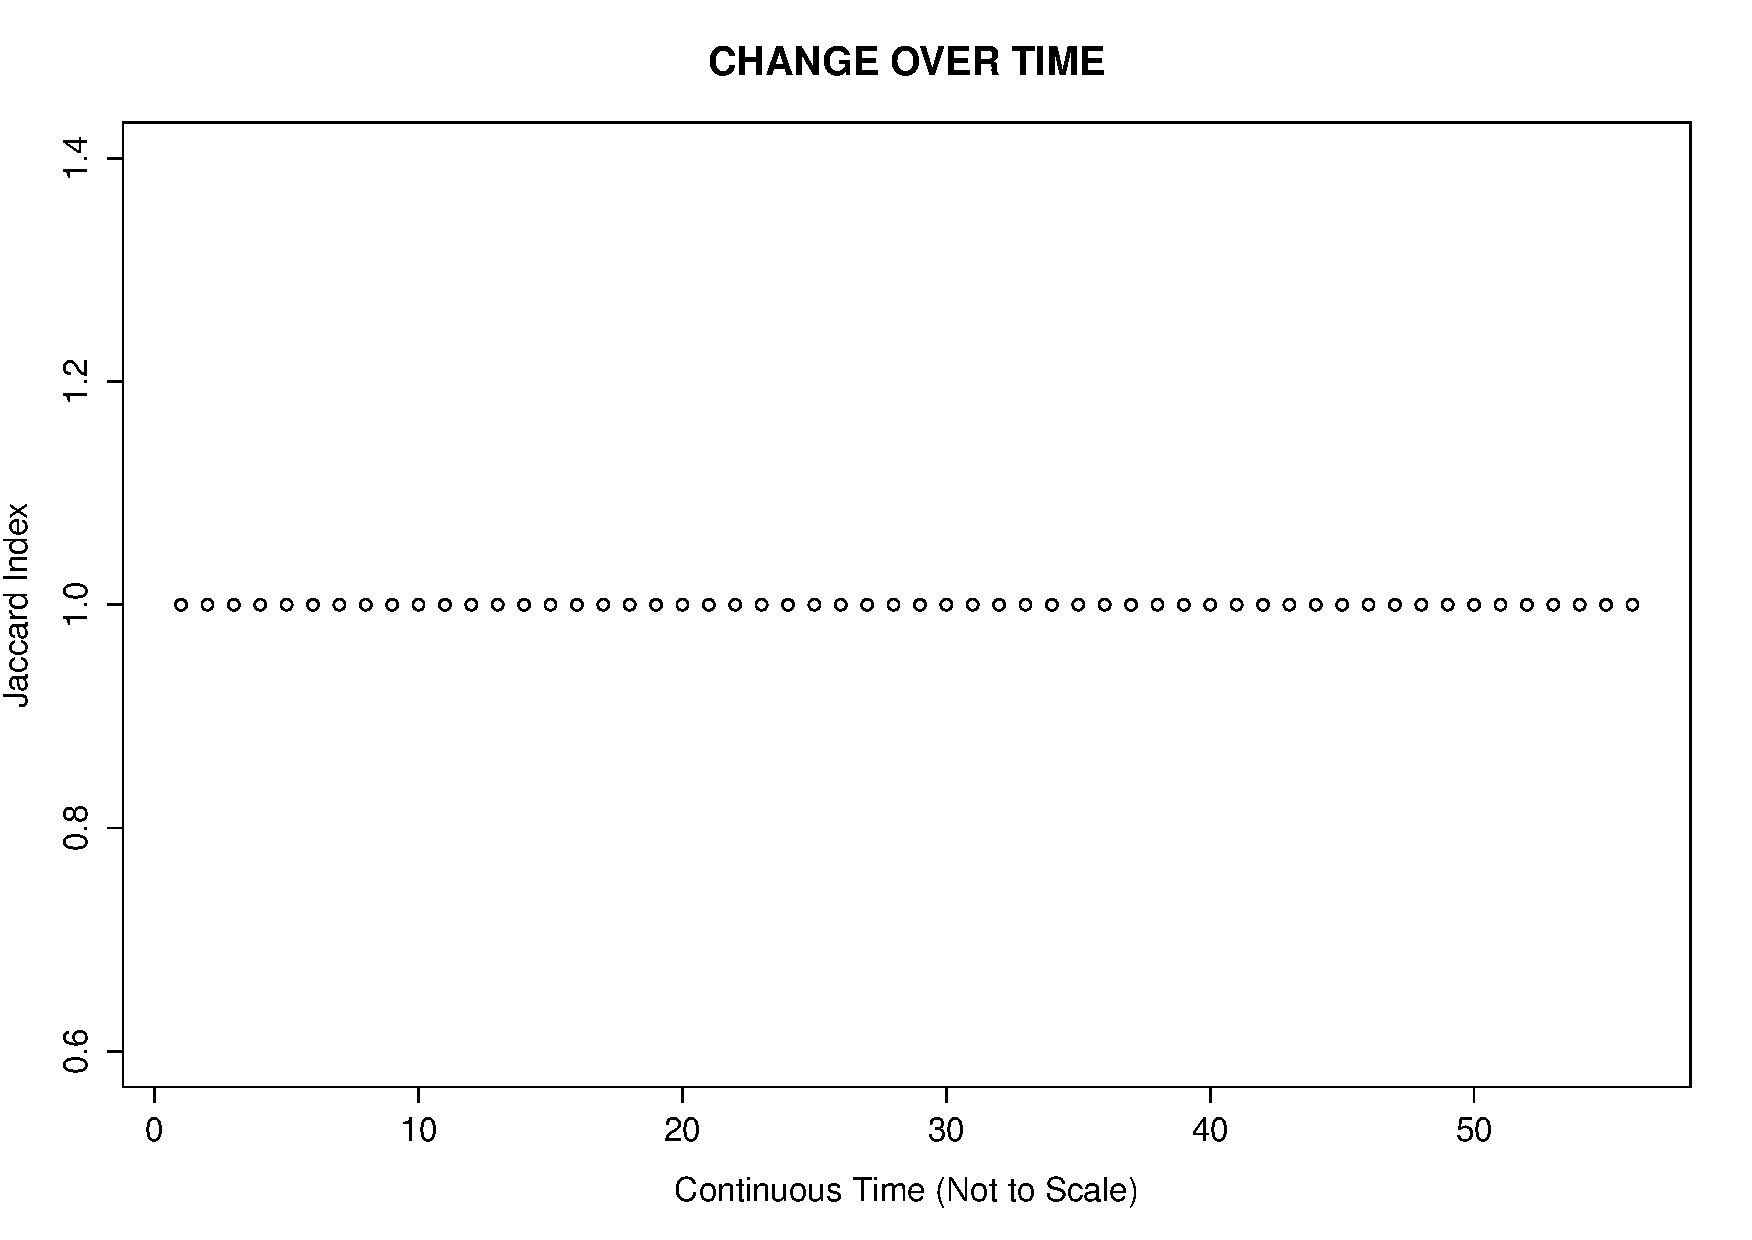
\includegraphics[width=0.8\columnwidth]{twelveth} % Example image
\end{center}

\begin{center}
{Figure 17: JACCARD INDEX Assuming Contant Time for Thirteenth URI}
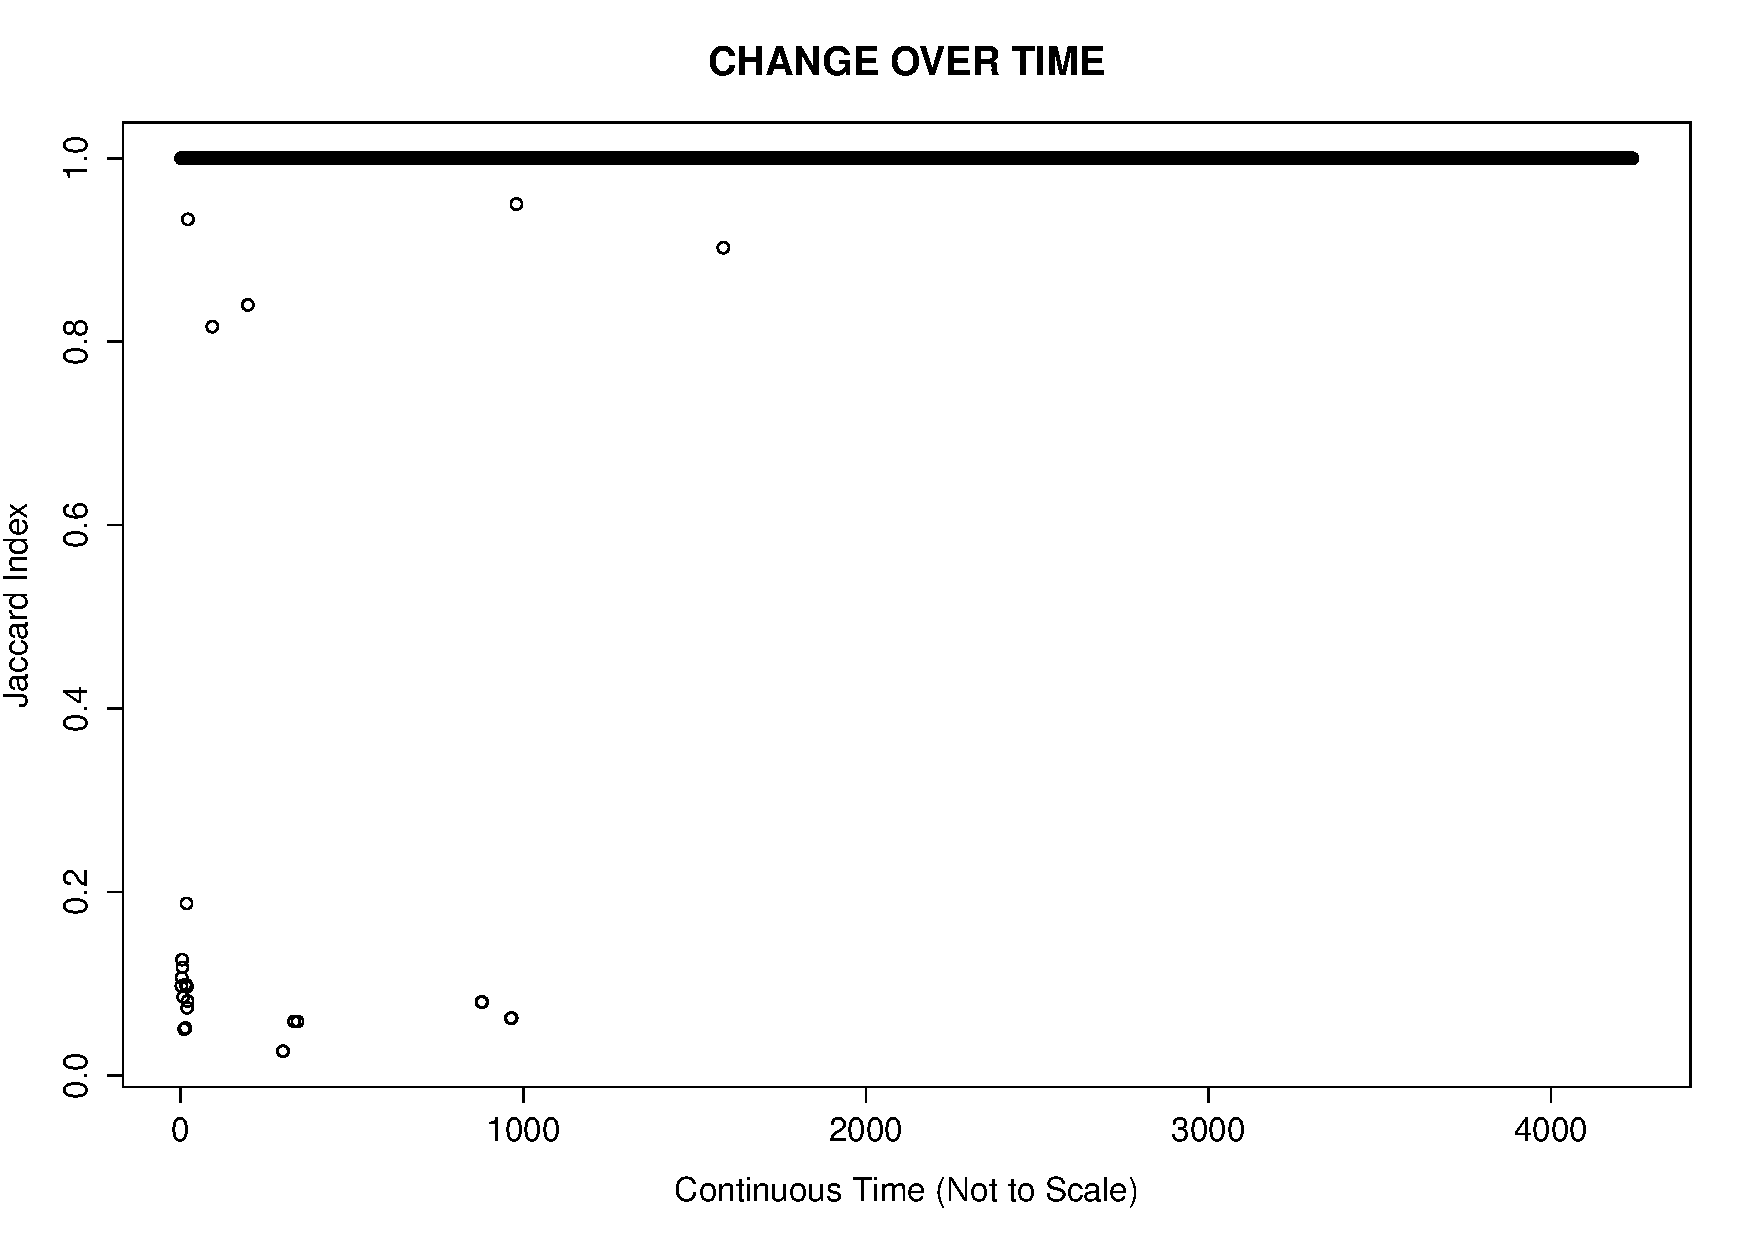
\includegraphics[width=0.8\columnwidth]{thirteenth} % Example image
\end{center}

\begin{center}
{Figure 18: JACCARD INDEX Assuming Contant Time for Fourteenth URI}
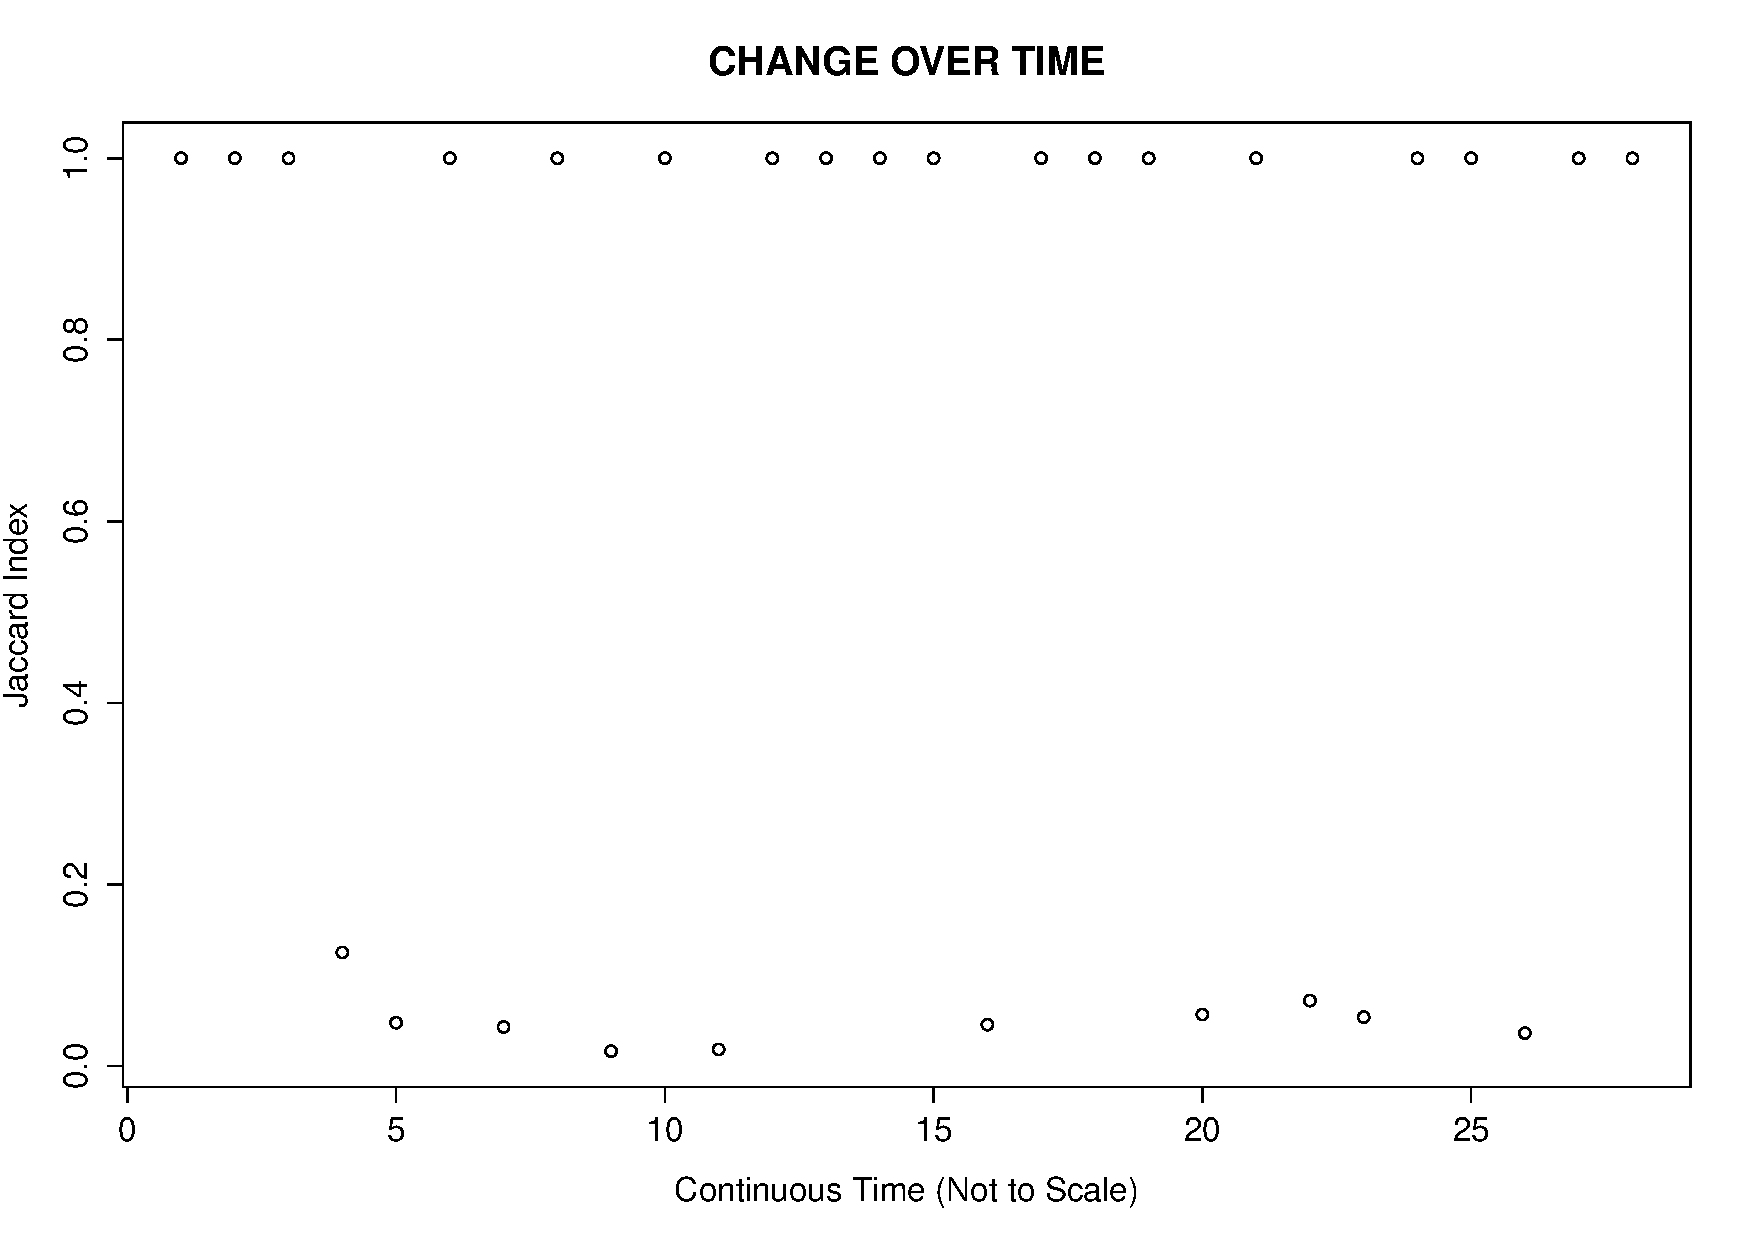
\includegraphics[width=0.8\columnwidth]{fourteenth} % Example image
\end{center}

\begin{center}
{Figure 17: JACCARD INDEX Assuming Contant Time for Fifteenth URI}
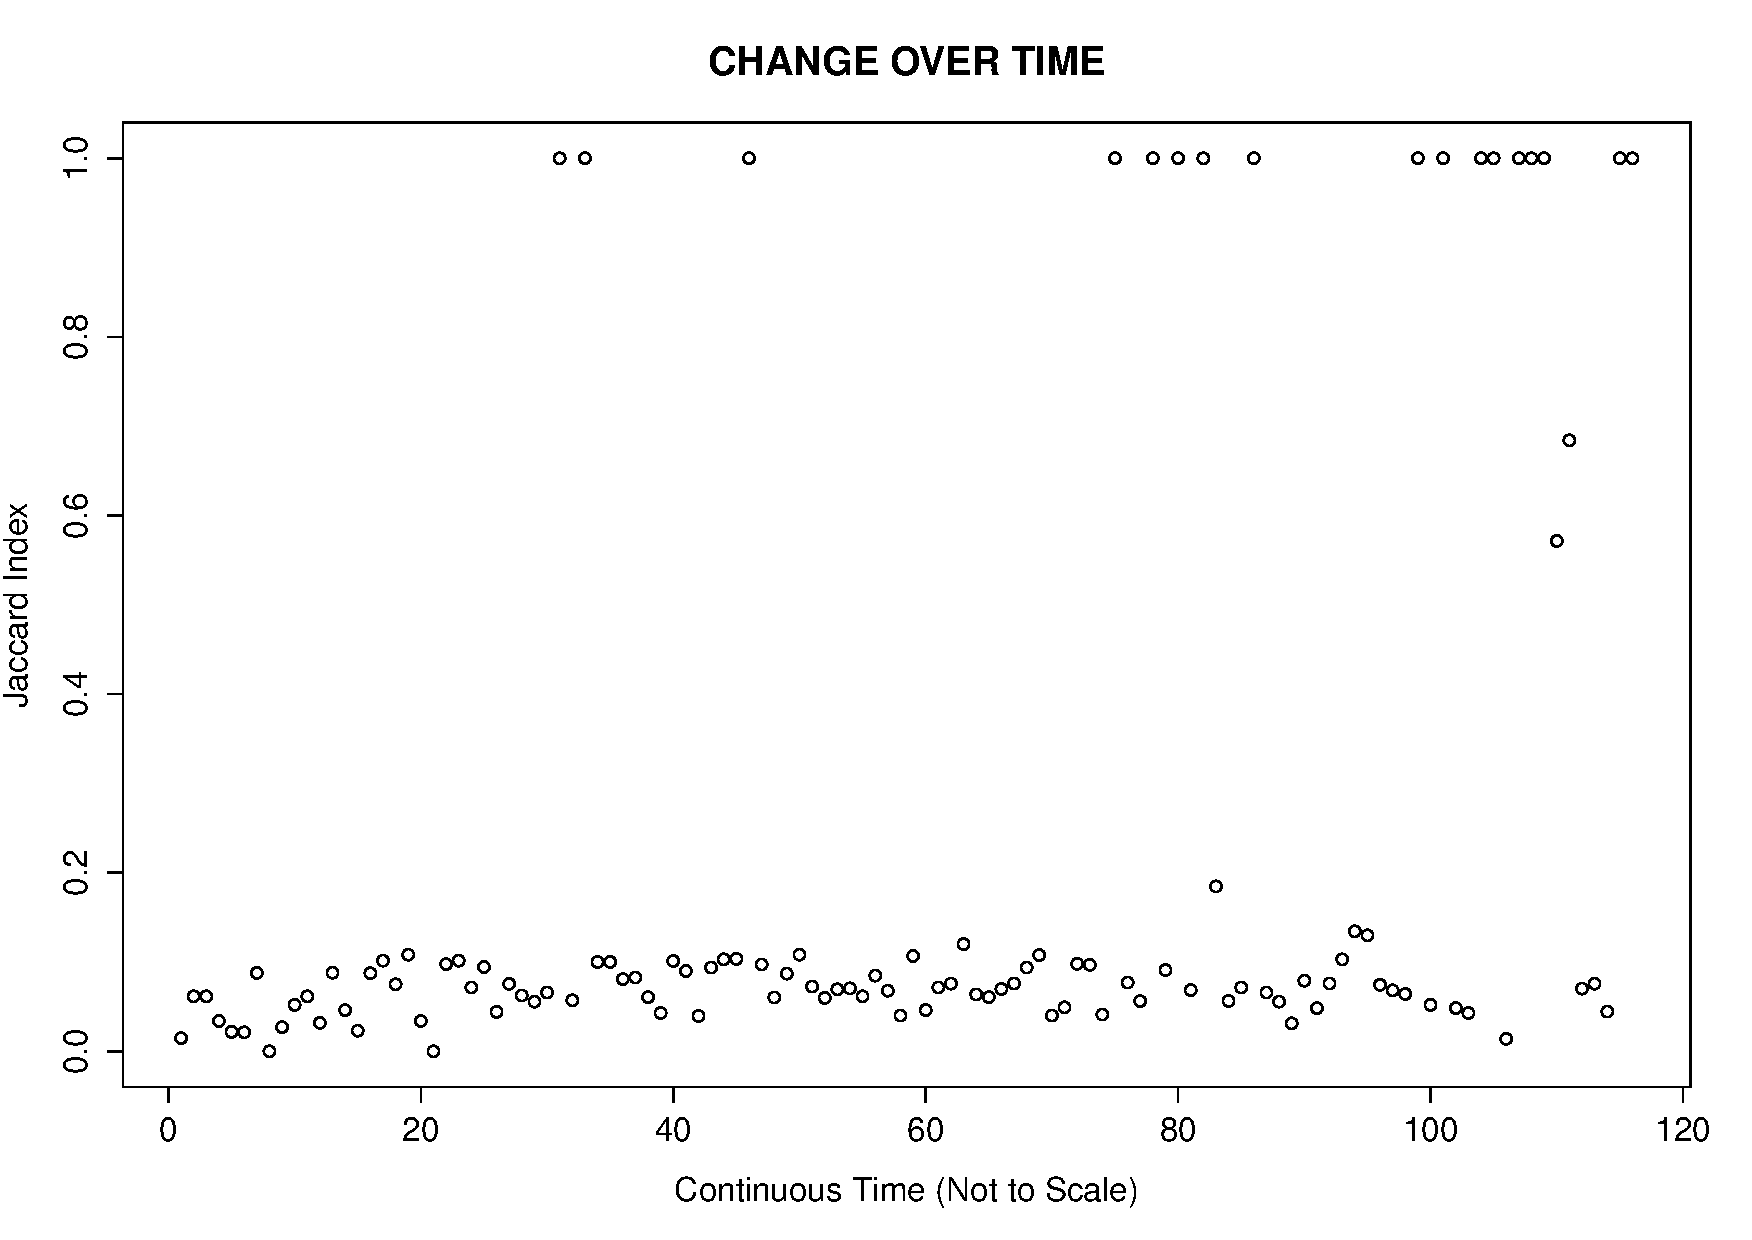
\includegraphics[width=0.8\columnwidth]{fifteenth} % Example image
\end{center}

CONCLUSION
\newline
For question 3 I was able to use 15 of 20 links that fulfilled the criteria, I also assumed a constant time and the jaccard index is placed in the same sequence as they occured, my intention was not to show the variations with respect to real(original) time of occurrence.

\end{homeworkProblem}


%------------------------------------------------------------------
%  Bibilography
%------------------------------------------------------------------
\bibliographystyle{plain}
\bibliography{assignment_4}
\nocite{*}
%----------------------------------------------------------------------------------------

\end{document}